\chapter{Detectors Test, Alignment and Calibration.} \label{analysis}

\paragraph{}
In this chapter we discuss the electronic test that have been carried out in the laboratory, and the calibrations needed in order to calculate, from the raw data, the quantities needed for the analysis.
The test in the lab consisted in checking the photo-multipliers tubes and the data acquisition electronics. The calibrations consist of determining the scaling factors required by the analysis program, to convert the raw data collected by the \textit{VFC}s to data in physical units. The important beam parameters are the impact point coordinates of the beam $X,Y$, the beam energy $E$, the beam current $I$ and the scattering angles $\theta_{x}$ and $\theta_{y}$. In the end, we discuss the auto-calibration procedure, which eliminates undesirable effects caused by the presence of an offset in the PMTs counts.

\section{Nino Board}

In this section we study the characteristics of the Nino board, which digitizes the signal from the PMTs. The NINO board has two parameters: \textit{Thr}, that controls the discriminator and \textit{Att}, which controls the attenuator circuit. These parameters are part of the settings of the DAQ program which controls the NINO board.
Because the values of \textit{Thr} and \textit{Att} are defined in arbitrary units, it is desirable to find a conversion formula to obtain the value of the threshold in physical units, as \SI{}{\milli \volt}.
Because of the NINO sensitivity to the input charge, it is not simple to define a unique value for the threshold in \SI{}{\milli \volt}, because the input charge of the detector signal depend on the shape, amplitude and time length. For example, signal with a large time and a small amplitude can generate the same charge with respect to narrow signal with high voltage amplitude. Despite this, some data have been acquired by the A1 collaboration, with which it is possible to define a raw conversion function from attenuation units to threshold. The idea behind  is to generate, with a wave generator, signals with fixed time length and shape, varying only the amplitude, and use them as input of the NINO board.
The data available were collected following this procedure. Unfortunately, these data were taken with an input signal shape that different from the signal shape of our experiment. We are aware that the conversion formula obtained with these data is only a rough estimation, however it can be useful to get an idea of the threshold values, in \SI{}{\milli \volt}.

\begin{figure}[hbtp]
\centering
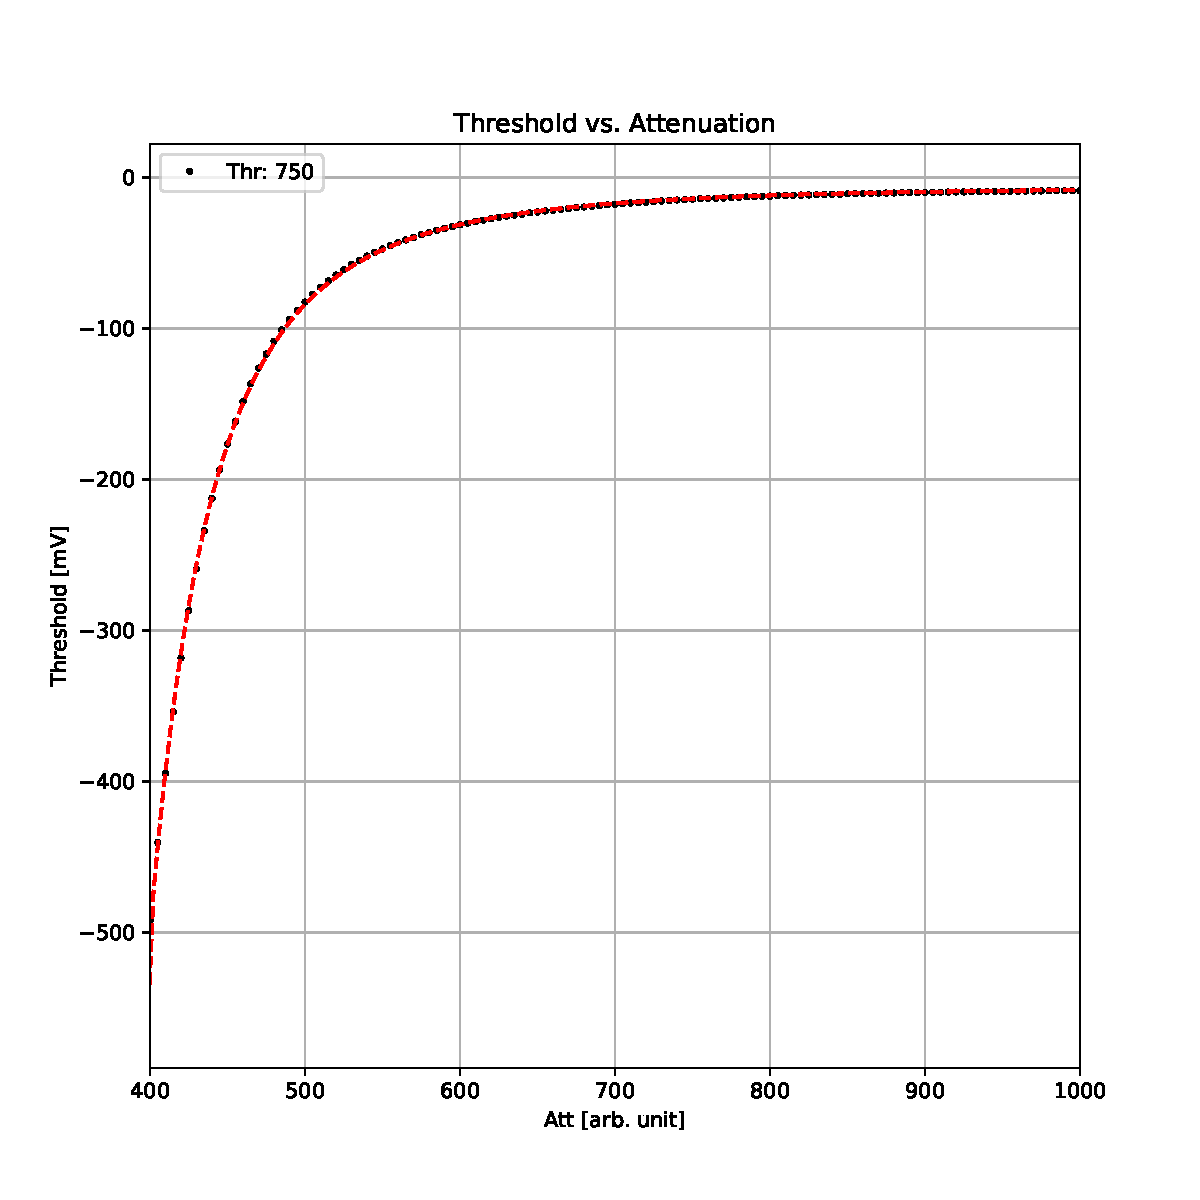
\includegraphics[scale=0.5]{Analysis/Calibrations/ThrvsAtt.pdf}
\caption{Threshold dependence versus attenuation. The input signals have a fixed shape and time length. The data are collected following this procedure: with a fixed amplitude of signal, the \textit{Att} is set to $4000$, the maximum, and decreased progressively, until the NINO board starts missing some pulses. All the data are acquired with a fixed value of \textit{Thr} = 750.} \label{fig:ThrvsAtt}
\end{figure}

The data shown represent the values of the amplitude of the input signals (in $\SI{}{\milli \volt}$) versus the values of \textit{Att}, and are taken for a fixed value of \textit{Att} = 750. The function used for the conversion is obtained from the fit of the data, the function used is the following: 

\begin{equation}
Threshold \, [\SI{}{\milli \volt}]= \dfrac{a}{(att - b)^{3}} + c
\end{equation}

The parameters of the formula are estimated using the function \textit{curve-fit} of the python library \textit{schipy}:

\begin{itemize}
\item $a = - 802111053 \, \frac{\SI{}{\milli \volt}}{[arb.unit]}$
\item $b = 382 \, [arb. unit]$
\item $c =  \SI{-6.1}{\milli \volt}$
\end{itemize}

As we can see, the relation between threshold and \textit{Att} is not linear. Around the values $400$ - $700$ we observe large variability. For values higher than $700$, the threshold is low and almost constant. This mean that the attenuation, controlled by the attenuator in the input channel of the NINO board, is reduced progressively as 	\textit{Att} increases. 

\section{Detector Test}

Before the beam time, some test with the two detectors were performed, to check that the PMTs were still working after some years of inactivity, and that the new electronics was able to count properly the pulses and store the data. For this studies, we didn't have a radioactive sources to employ. Anyway the signal shape using radioactive sources is expected to be different from signal of the $\SI{570}{\mega \electronvolt}$ electrons used in the experiment. The typical energies of nuclear decay are in the order of $E \simeq \SI{1}{\mega \electronvolt}$,  with consequently only a small production of Cherenkov light, difficult to detect. A different approach is followed, using cosmic rays rate as a probe. 
The cosmic rays are able to produce Cherenkov light in the fused-silica bars, since the refractive index is $n = 1.45$, and a particle emits Cherenkov light when its $\beta = \frac{v}{c}$ is more than $\frac{1}{n} = 0.69$. The principal component of the cosmic rays at sea level is made by muons, produced in the electromagnetic and hadronic showers in high atmosphere. The energy of the muons reaching sea level is about $\SI{4}{\giga \electronvolt}$, $\beta$ for these particles is:

\begin{equation}
\beta_{\mu} = \dfrac{p}{E} = \dfrac{\sqrt{E^{2} - m_{\mu}^{2}}}{ E^{2}} \simeq 0.99
\end{equation}

The muons are relativistic and their speed is over the threshold for Cherenkov light production. Knowing that the expected number of event for cosmic rays is about $1 \frac{event}{\SI{}{\centi \meter\squared} \SI{}{\minute}}$ we can compute the expected values for the number of events. We decided to take 1 minute long acquisition for both the two detectors, this leads to $70$ expected events for detector B  and  $210$ events for detector A. These values are a rough estimate, because the effective area seen by the each PMT is less than the total area of the fused-silica bar. The rates measured in the laboratory are $\simeq 60$ for detector B and $\simeq 100$ for detector A.     
The first step is to select a good work point for the threshold. So, fixing the value of the threshold parameter for the NINO board, we took several acquisitions, each of them one minute long, increasing the attenuation (figure \ref{fig:AttB}). We powered the PMTs with a negative voltage around $\SI{-1000}{\volt}$, as suggested in the data-sheet, and covered the Cherenkov detector with a shielding blanket, to avoid ambient light simulating a signal.

\begin{figure}[!ht]
\centering
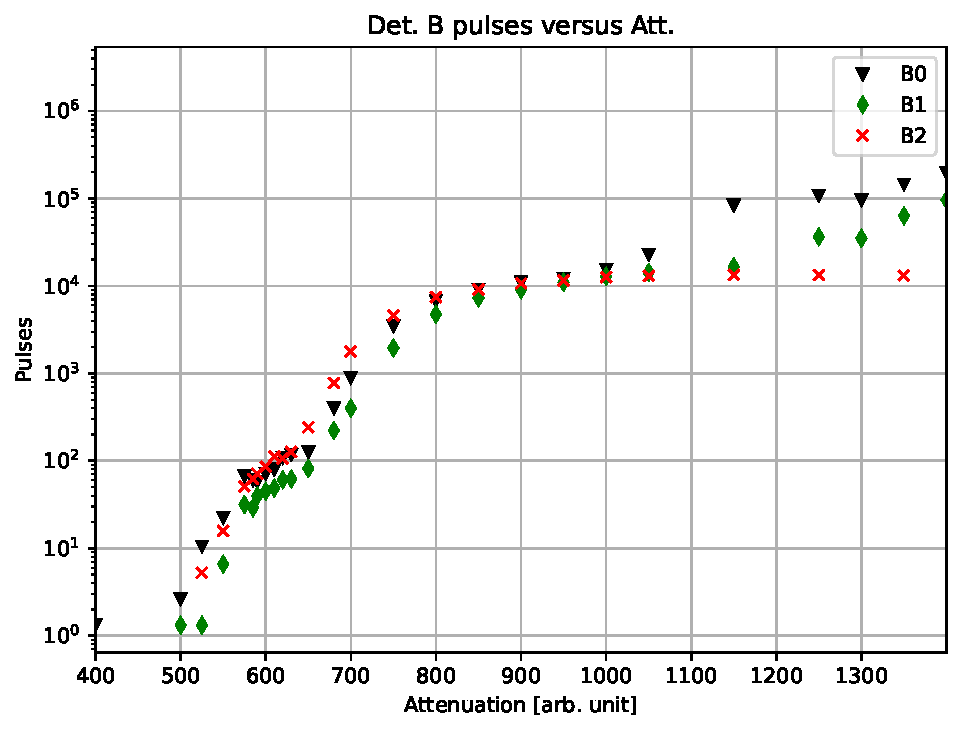
\includegraphics[width = 0.85\textwidth]{Analysis/AttenuationB.pdf}
\caption{Attenuation scan for Detector B.}
\label{fig:AttB}
\end{figure}

We observed a small knee, around the zone of 580 − 600 of \textit{Att}, where the number of counts was almost constant, roughly equal to the number of expected events from muons hitting the detector. Then we observe a big edge for attenuation = 700. Looking at the plot \ref{fig:ThrvsAtt}, we assume that the attenuation values are so high that electronic noise is no longer rejected, in fact the counts grow enormously. The \textit{Att} was set at 600 as a starting point for the experiment.
Once the attenuation is set, we have studied the statistical fluctuation of the counts. 10 acquisitions, each of them \SI{1}{\minute} long are collected and reported in table \ref{tab:CountB}.

\begin{table}[!htb]
\centering
\begin{tabular}{l|c|c|c}
\hline 
$n^{\circ}$ acquisition & B0 & B1 & B2 \\
\hline 
1 & 58 & 60 & 62 \\  
2 & 62 & 55 & 59 \\ 
3 & 61 & 59 & 70 \\ 
4 & 73 & 66 & 70 \\ 
5 & 68 & 66 & 56 \\ 
6 & 59 & 52 & 64 \\ 
7 & 69 & 74 & 77 \\
8 & 48 & 49 & 57 \\ 
9 & 70 & 54 & 58 \\ 
10 & 60 & 61 & 66\\
\hline
\end{tabular} 
\caption{Detector B counts for $10$ acquisition of $\SI{1}{\minute}$ long, with \textit{Att} equal to 600.}
\label{tab:CountB}
\end{table}

These data are interesting, we can check if the counts are following the theoretical distribution of the events expected for cosmic rays at sea level. If the PMTs are working well, we know that the number of counts should be Poisson-distributed:

\begin{equation}
Pdf(\mu,k) =  \frac{\mu^{k}}{k!} e^{-\mu}
\end{equation}

The variance of the Poisson distribution is equal to the mean of the counts, and we expect the same behaviour also for the sample mean and the sample variance, the values are computed and reported in table \ref{tab:Bcounts}

\begin{table}[ht]
\centering
\begin{tabular}{l|c|c|c}
\hline 
PMT & $\mu$ & $\sigma^{2}$ & Correlation $C_{ij}$ \\
\hline
1 	& 62.8	& 54.4	& $C_{11} = 0.66$\\
2 	& 59.6	& 57.2	& $C_{23} = 0.65$\\
3	& 63.9	& 47.0  & $C_{13} = 0.35$\\
\hline
\end{tabular}
\caption{Mean, variance and correlation coefficient for detector B and PMT in overlap.}
\label{tab:Bcounts}
\end{table}

We report also the correlation $C_{ij}$ between the PMTs. The result are fine: we are able to see a positive correlation between adjacent PMT, and as expected the correlation is lower in the case of the more distant. This is explained by the lower probability that the photons of Cherenkov radiation light up at the same time PMTs that are far away from each other.
We can test that the data follow a Poisson distribution using the well-known Gosset test, defined as:

\begin{equation}
\chi^{2}_{n-1} = \sum_{i = 1}^{n} \dfrac{(Obs_{i} - Exp_{i})}{Exp_{i}}
\end{equation}

where $Obs$ are the observed counts, and $Exp$ are the expected counts.
We report the results for detector B in table \ref{tab:GossetB}. The test shows that there is good agreement with the hypothesis that the counts are Poisson-distributed.

\begingroup
\setlength{\tabcolsep}{8pt} % Default value: 6pt
\renewcommand{\arraystretch}{1.2} % Default value: 1
\begin{table}[htb]
\centering
\begin{tabular}{c|c|c|c}
\hline 
Pmt: & 1 & 2 & 3 \\ 
\hline
$\chi^{2}_{9}$ & 8.52 & 8.45 & 6.37 \\ 
\hline
\end{tabular}
\caption{Gosset test for detector B}
\label{tab:GossetB} 
\end{table}
\endgroup

At this point, to convince oneself that the detector B is measuring signals given by the passage of cosmic rays, and not only noise, a fourth PMT (a spare component left in the lab) was used. This other PMT was coupled to a small block of fused silica (\SI{5}{\centi \meter} $\times$ \SI{5}{\centi \meter}), and was placed in overlap with detector B, roughly in correspondence of B2. A first check was to look for coincidence signals at the oscilloscope, between detector B and the PMT in overlap.

\begin{figure}[!ht]
\centering
\includegraphics[width = 0.4\textwidth]{Analysis/IMG_20221027_170925.jpg} 
\caption{Coincidence signal between PMTs B0 and B2 acquired with the oscilloscope.}
\label{fig:CoincidenceSignal}
\end{figure}

Then we have acquired 10 acquisition one minute long, as before, measuring the counts of detector B and a PMT in overlap. Unfortunately, the DAQ is not designed to take coincidences, so a different procedure was followed to check is the PMTs are triggered by the same passage of particles. 
The correlation coefficient between the PMT in overlap and the detectors is a good statistic for this purpose: if a positive correlation between the counts is observed, then a certain number of signals is triggered by the same passage of particles. The result for detector B are reported in table \ref{tab:OverlapB}:

\begin{table}[ht]
\centering
\begin{tabular}{lcccl}
\hline 
$n^{\circ}$ acquisition  & B0 & B1 & B2 & $Ov$ \\ 
\hline 
1 & 63 & 57 & 72 & 28 \\ 
 
2 & 55 & 51 & 64 & 18 \\ 
 
3 & 62 & 53 & 75 & 27 \\ 
 
4 & 71 & 62 & 75 & 33 \\ 
 
5 & 68 & 59 & 49 & 23 \\ 
 
6 & 57 & 55 & 63 & 18 \\ 
 
7 & 70 & 64 & 64 & 24 \\ 
 
8 & 50 & 69 & 69 & 25 \\ 
 
9 & 65 & 62 & 62 & 19 \\ 
 
10 & 74 & 71 & 77 & 28 \\ 
\hline
\end{tabular} 
\caption{Detector B counts for 10 acquisitions of $\SI{1}{\minute}$ long, with PMT $Ov$ in overlap.}
\label{tab:OverlapB}
\end{table} 

The sample mean, the variance and the correlation between the detector B and the PMT in overlap are reported in table \ref{tab:ResultBB}. The result for the Gosset test are reported in table \ref{tab:GossetForOver}.

\begin{table}[ht]
\centering
\begin{tabular}{c|c|c|c}
\hline 
PMT & $\mu$ & $\sigma^{2}$ & Correlation \\
\hline
1 	& 63.5	& 58.9	& 0.49 \\
2 	& 60.3	& 43.3	& 0.38 \\
3	& 67.0	& 71.1  & 0.65 \\
\hline
\end{tabular}
\caption{Mean, variance and correlation coefficient for detector B and PMT in overlap.}
\label{tab:ResultBB}
\end{table}

A positive correlation is measured for all the PMTs of detector B. This indicates that a certain amount of signal are detected simultaneously.

\begingroup
\setlength{\tabcolsep}{8pt} % Default value: 6pt
\renewcommand{\arraystretch}{1.2} % Default value: 1
\begin{table}[ht]
\centering
\begin{tabular}{c|c|c|c|c}
\hline 
   & B0 & B1 & B2 & PMT in overlap \\ 
\hline
$\chi^{2}_{9}$ & 8.95 & 6.44 & 10.96 & 9.52\\ 
\hline
\end{tabular}
\caption{Gosset test for detector B and the PMT in overlap, for the 10 acquisition in table \ref{tab:OverlapB}}
\label{tab:GossetForOver}
\end{table}
\endgroup

The same procedure was followed also for detector A (see figure \ref{fig:ScatDetA}). We analyzed 4 signal at a time, because during these lab test we had only one NINO board, with only 4 channels available. The tests for the set of PMTs (A7,A6,A5,A4,A3) showed good result: the distribution of the counts was in agreement with the expected and the correlation coefficient between nearby PMTs and the PMT is overlap was different from zero and positive. For the set of PMTs (A2,A1,A0), some issues have emerged. Primarily the counts did not vary during the scan in \textit{Att} and this has made impossible to identify a value for the \textit{Att}. To study the behaviour of the counts, once again 10 acquisitions were acquired, and are reported in table \ref{tab:PmtAproblem}. \newpage

\begin{table}[htb]
\centering
\begin{tabular}{lcccc}
\hline 
$n^{\circ}$ acquisition & A2 & A1 & A0 & $Ov$ \\ 
\hline 
1 & 91 & 51 & 50 & 27 \\ 
 
2 & 86 & 61 & 50 & 7 \\ 
 
3 & 58 & 48 & 45 & 18 \\ 
 
4 & 95 & 62 & 41 & 29 \\ 
 
5 & 69 & 60 & 50 & 21 \\ 
 
6 & 85 & 57 & 45 & 19 \\ 
 
7 & 66 & 51 & 46 & 28 \\ 
 
8 & 74 & 51 & 48 & 22 \\ 
 
9 & 77 & 43 & 45 & 17 \\ 
 
10 & 62 & 44 & 50 & 29 \\ 
\hline 
\end{tabular}
\caption{PMTs A2,A1,A0 counts for 10 acquisition of \SI{1}{\minute} long.}
\label{tab:PmtAproblem}
\end{table}

The mean, variance and correlation between the PMTs counts is reported in table \ref{tab:ResultAA}:

\begin{table}[!ht]
\centering
\begin{tabular}{lccc}
\hline 
PMT & $\mu$ & $\sigma^{2}$ & Correlation \\
\hline
2 	& 76.3	& 160	& $C_{21}$ = 0.55 \\
1 	& 52.8	& 47.5	& $C_{10}$ = -0.10 \\
0	& 47.0	& 9.6   & $C_{20}$ = -0.22 \\
\hline
$Ov$ & 21.7 & 48.2 & \\
\hline
\end{tabular}
\caption{Mean, variance and correlation coefficient for detector A and PMT in overlap.}
\label{tab:ResultAA}
\end{table}


The variance $\sigma^{2}$ for A0 and A2 are quite different from the expected mean $\mu$. The Gosset test for this data are reported in table: \ref{tab:GossetA0A1A2} 

\begingroup
\setlength{\tabcolsep}{8pt} % Default value: 6pt
\renewcommand{\arraystretch}{1.2} % Default value: 1
\begin{table}[!ht]
\centering
\begin{tabular}{c|cccc}
\hline 
Pmt: & A2 & A1 & A0 & PMT in overlap \\ 
\hline
$\chi^{2}_{9}$ & 19.6 & 8.30 & 1.90 & 39.5\\ 
\hline
\end{tabular} 
\caption{Gosset Test for PMTs A2,A1,A0 of detector A.}
\label{tab:GossetA0A1A2}
\end{table}
\endgroup
\smallskip

The expected error for the result of this test is $\sigma = \sqrt{2 \cdot (n-1)} \simeq 4$. In this case we are observing 3 values that are more than  $3 \cdot \sigma$ far from the expected value. If we look at the correlation matrix :

\begin{table}[!h]
\centering
\begin{tabular}{ccccc}
\hline 
pmt: & $Ov$ & 0 & 1 & 2 \\ 
\hline 
$Ov$ & 1 & -0.18  & -0.21  & -0.06  \\ 
0 	 & -0.18  & 1 & -0.10  & -0.22  \\ 
1    & -0.21  & -0.10  & 1 & 0.56  \\ 
2    & -0.06 & -0.22  & 0.56  & 1 \\ 
\hline 
\end{tabular}
\caption{Correlation coefficient between the PMTs (A2,A1,A0) and the PMT in overlap.}
\end{table}

We observe negative correlation between the pmts, something not expected. After some investigations, we find out that the program which controls the NINO board had a bug: the program partially overwrote some detector B settings for detector A as well. Since detector B has only three pmt's, the problem affected the PMT's with the same numbering as detector A. After fixing this issue we repeated the same test, without finding any problem. 

\begin{figure}[!htb]
\centering
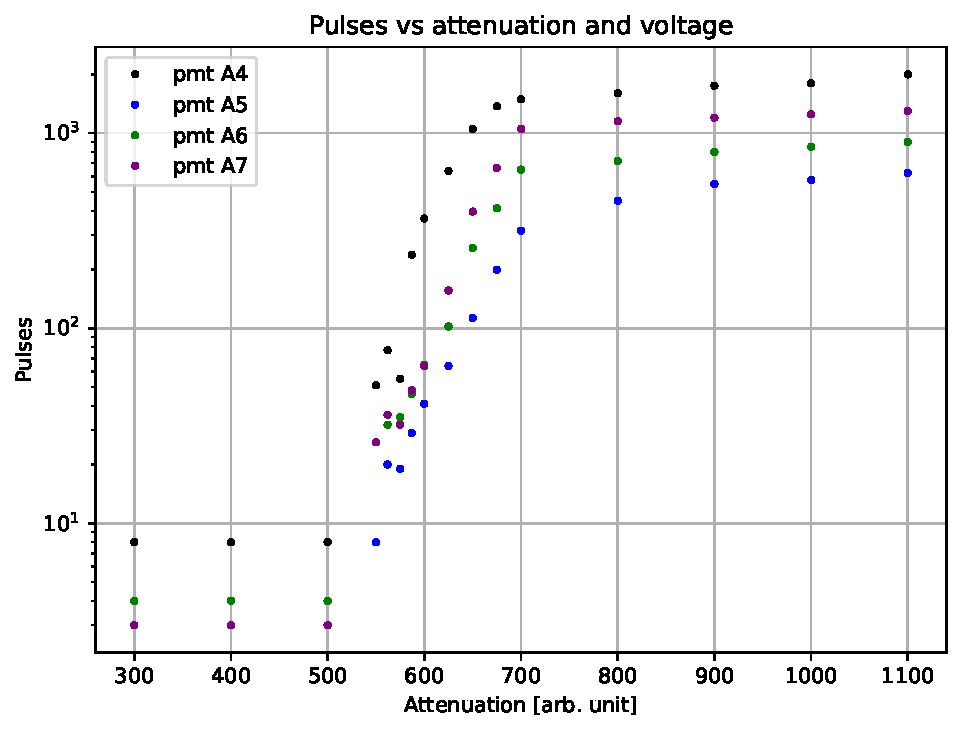
\includegraphics[width = 0.75\textwidth]{Analysis/AttenuationA(4-7).pdf}
\caption{Attenuation scan for Detector A, for the pmt 4-5-6-7}
\label{fig:ScatDetA}
\end{figure}

\newpage
\section{Calibration}

For the transverse asymmetry on $^{12}C$ represent an ideal test for the new electronic system. Previous measurements of the $A_{n}$ have been performed at MAMI for carbon target (\cite{Esser:2018vdp}). For this experiment, the red spectrometer is placed at the angle of $+22.5^{\circ}$, and the blue one at $-22.5^{\circ}$, with respect to the longitudinal direction. For these two angle, we have the same kinematics and $Q^{2}$ values of the previous measurement. The $Q^{2}$ value was measured for a low current beam ($I = \SI{5}{\nano \ampere}$) with the spectrometers detectors. The $Q^{2}$ values are reported with and without rejecting the inelastic scattered electrons. The inelastic scattered electrons are rejected imposing an energy threshold. 

\begin{flushleft}
\begin{align*}
& det. A : \qquad Q^{2} = \SI{0.041}{\giga \electronvolt \squared} \qquad \textnormal{without Cut} \\
& det. A : \qquad Q^{2} = \SI{0.039}{\giga \electronvolt \squared} \qquad \textnormal{with Cut} \\
& det. B : \qquad Q^{2} = \SI{0.041}{\giga \electronvolt \squared} \qquad \textnormal{without Cut} \\
& det. B : \qquad Q^{2} = \SI{0.041}{\giga \electronvolt \squared} \qquad \textnormal{with Cut} 
\end{align*} 
\end{flushleft}

The $Q^{2}$ values are the same of the last measurement performed at MAMI, and are measured with and without rejecting the inelastic electrons. 

\subsection{Alignment of the Scattering Plane.}

The scattered electrons are deflected upward by the magnetic field inside the spectrometers A and B. However, the spectrometer detectors and systems are not directly used to measure the transverse asymmetry, due to the high current intensity, which would damage the electronics.
Consequently, the scattered electrons are measured by the detectors A and B, described in section \ref{detectors}, which are installed between the drift chamber and the scintillator panel (see figure \ref{fig:internal}) of the spectrometers. At the start of the experiment, the scattered particles must be aligned to the fused-silica bars.
This procedure is performed using a low current mode of the beam ($I = \SI{5}{\nano \ampere}$). For this mode the spectrometer systems can be used to detect the particles. Since the position of our detector A and B  inside the spectrometers is known, we can use the Cherenkov detector to visualize where the electrons. Changing the configuration of the magnetic field, the electrons trajectory is oriented in such a way that is intersects the detectors A and B. For detector A the scattered electron beam has been aligned to pass over the fused silica in correspondence of PMT A7, therefore this PMT measures higher rates. For detector B the same procedure was done, aligning the scattered beam in correspondence of PMT B0. Once the alignment is done, we turned off the spectrometers system, performing the other necessary calibrations with the detector A and B. 

\subsection{Beam Monitor Calibration, XY Monitor} \label{XYpos}

The values measured by the beam monitors are digitalized by the VFCs. The analysis program converts the raw counts in voltage values with the formula shown in equation \ref{eq:Vfc}. For the calibration of the XY position monitors, special targets are used. In the target frame (see figure \ref{fig:targetFrame}) there are two targets made by three carbon wires that are mounted at a known distance from each other, horizontally and vertically aligned. 

\begin{wrapfloat}{figure}{I}{0.5\textwidth}
\centering
\includegraphics[width = 0.45\textwidth]{ExperimentalSetup/target.pdf}
\caption{\label{fig:targetFrame} Target frame, on the top the three carbon wires that are used to calibrate the positions monitors. Then the carbon target and two lead targets.}
\vspace{-0pt}
\end{wrapfloat}

The distance between the center of the two external wires is measured, to be $ d_{horizontal} = \SI{2.38}{\milli \meter}$ for the horizontal wires and $d_{vertical} = \SI{2.33}{\milli \meter}$ for the vertical wires. The procedure to measure the scaling factor used to convert from the raw-data in $\SI{}{\volt}$ to $\SI{}{\micro \meter}$, is the following: we ask MAMI operators to gradually shift the beam position, in the horizontal direction horizontal wire target and in the vertical direction for the vertical target. The beam position is changed by varying the magnetic field produced by the \textit{Wobbler 16} magnets (see figure \ref{fig:BeamLine}). During the position shift, the detectors measure the rate of scattered electrons, that increases when the beam hits one of the three wires and decreases when the beam is centered between two wires. We plot the detector counts versus the $XY$ monitors values, in voltage, and we estimate the position of the two external peaks. This values can be used, together with the distance $d_{horizontal},d_{vertical}$ already measured, to compute the scaling factors. This procedure is repeated for $X21/Y21$ and $X25/Y25$ monitors. We plot the PMT rate versus the $X25,X21,Y25,Y21$, given in $\SI{}{\volt}$. 
To identify the three peaks of the carbon target, we fit the data using a gaussian model (see figure \ref{fig:HorizontalCalibration}). The mean $\mu$ represents the center of the wire, given in $\SI{}{\volt}$.
We assume that the beam travels in a straight line beginning at the \textit{Wobbler 16} magnet, that in our convection is the origin of coordinate system, with the $z$ axis oriented toward to the target (left direction in the beam scheme).
\begin{figure}[hbtp]
\centering
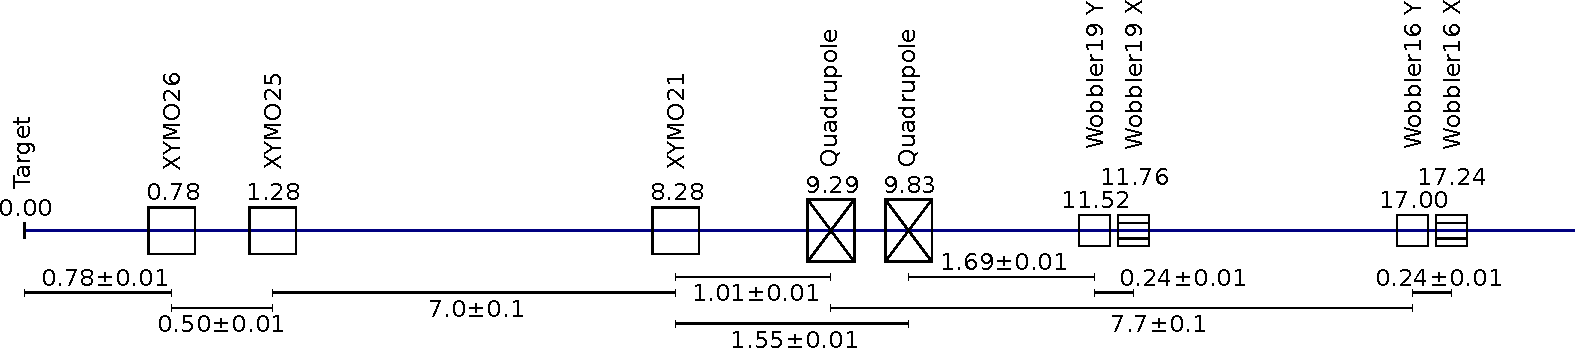
\includegraphics[width = 0.75\textwidth]{figures/XYMOCalibBeamLine.pdf}
\caption{Beam line scheme.}
\label{fig:BeamLine}
\end{figure} 

The Beam parameters are measured by the Monitors $X/Y_{21}, X/Y_{25}$, which are located at some distance with respect to the target. For the $Y_{25}$ monitor (the procedure is the same for the others) the beam $y$ position is described by:

\begin{align*}
Y_{beam} = m \cdot (Z_{Y25})
\end{align*}

Where $Z_{Y25}$ is the longitudinal distance between the \textit{wobbler16} magnet and the $Y25$ monitor. From the scheme \ref{fig:BeamLine}, the longitudinal distance between $Y_{25}$ monitor and the \textit{wobbler16} magnet is $\SI{1.57}{\meter}$. The Position on the target is given by $Y_{target} = m \cdot Z_{target}$. The scaling factor is given by:

\begin{equation}
c_{Y25} = \dfrac{d_{vertical} [\SI{}{\milli \meter}]}{ Y_{target}} 
\end{equation}

where $c_{Y25}$ indicates the scaling factor of the monitor. This procedure is repeated for all the monitors, and the scaling factor $c_{Y25}$, $c_{Y21}$ , $c_{X25}$, $c_{X21}$ are measured. The analysis program uses these quantities to compute the beam position on the target, and from that the incident angles with respect to the $X,Y$ directions, which are needed for the analysis.

\begin{figure}[hbtp]
\centering
\subfloat[][]{
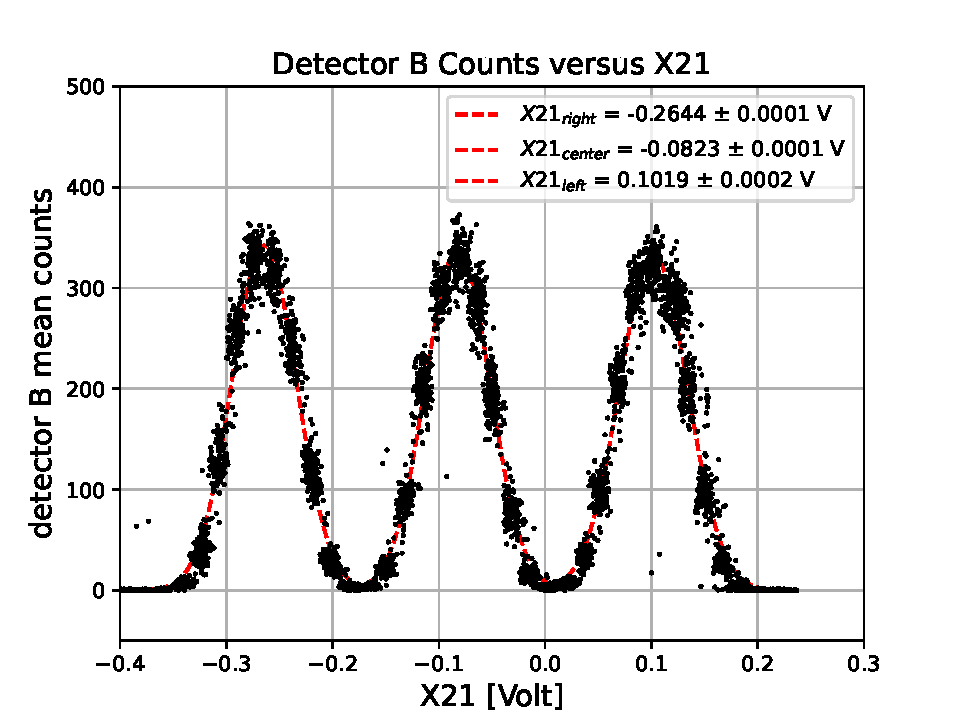
\includegraphics[width=0.4\textwidth]{Analysis/HorizontalCalibration.pdf}}
\subfloat[][]{
\includegraphics[width=0.4\textwidth]{Analysis/HorizontalCalibrationX25.pdf}}
\caption{Plot of the averaged count of detector B, with the slow variations of the beam position in the horizontal direction. The three peaks occur when the beam is aligned with the center of the wire. The values on the X axis are in $\SI{}{\volt}$}
\label{fig:HorizontalCalibration}
\end{figure}

The analysis program calculate $X$ and $Y$ values in \SI{}{\micro \meter}, combining the values measured by the two monitors (see figure \ref{fig:BeamTraje}).

\begin{figure}[!hbtp]
\centering
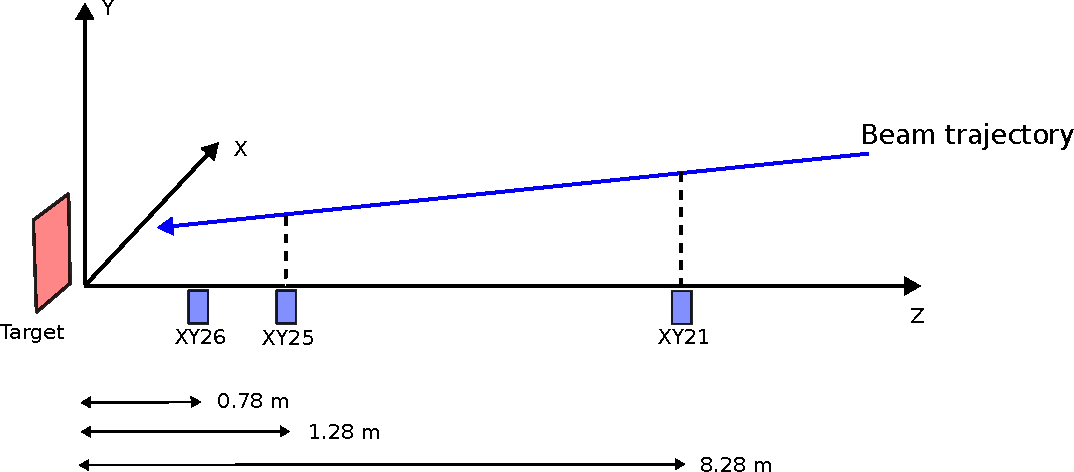
\includegraphics[scale=0.75]{Appendix/scheme.pdf}
\caption{Figure of the beam trajectory, the position $X$ and $Y$ are measured by the monitors (blue boxes). Assuming a linear motion of the particles, the hitting positions on the target are computed.}
\label{fig:BeamTraje}
\end{figure}

The functions used are implemented considering a reference system with the origin coincident to the center of the target, and the $Z$ axis oriented towards the \textit{Wobbler16} magnet. The beam trajectory is described by the following equation:

\begin{align*}
y &= m_{y} \cdot z + q_{y} \\
x &= m_{x} \cdot z + q_{x}
\end{align*}

$q_{x}$ and $q_{y}$, that are the intercepts, are the desired quantities.
Imposing in the above equations the passage through the points ($Z_{25}$;$X_{25}$) and ($Z_{21}$;$X_{21}$) (identical procedure for $Y$) we can resolve the system for $q_{x}$, obtaining:

\begin{equation}
q_{x} = \dfrac{Z_{25} \cdot X_{21} - Z_{21} \cdot X_{25}}{Z_{25} - Z_{21}}
\end{equation} 

the solution for $q_{y}$ is identical. The scattering angles $\theta_{x}$ and $\theta_{y}$ are instead related to the slope $m$, knowing that $tan(\theta) = m$. The angles are given by the formula:

\begin{equation}
\theta_{x} = \dfrac{X_{25} - X_{21}}{Z_{25} - Z_{21}}
\end{equation}

To check that the functions are well implemented, we plot in figure \ref{fig:CheckHori} the PMTs counts versus the $X$ beam position on the target. the distance between the two external peaks, reported in the plot, is in agreement with the expected distance $d_{x}  = \SI{2.38}{\milli \meter}$.
 
\begin{figure}[hbtp]
\centering
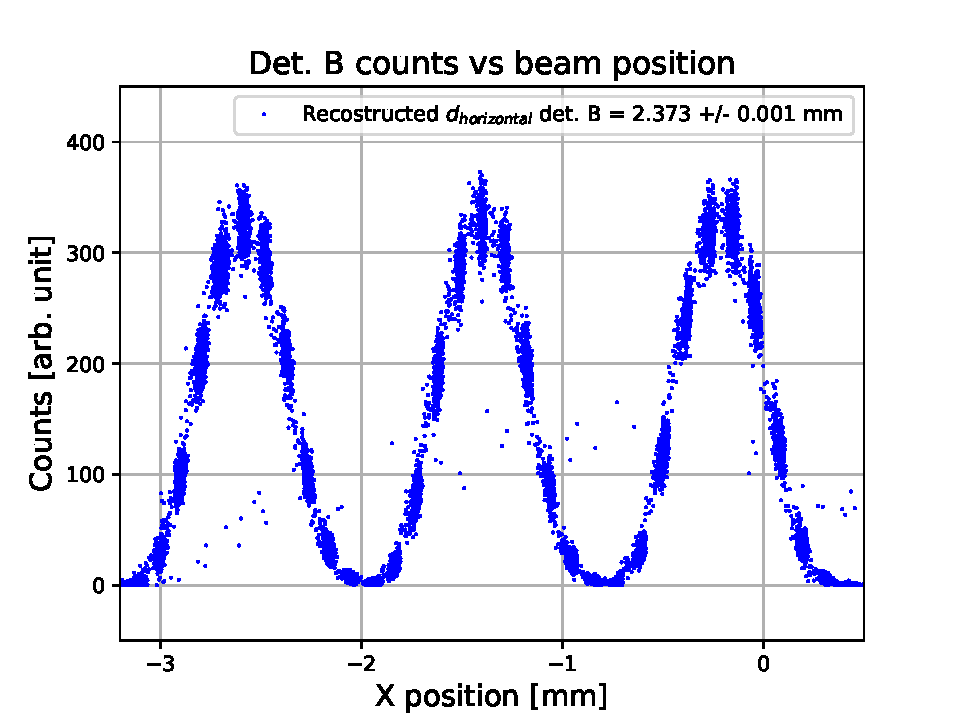
\includegraphics[width=0.45\textwidth]{Analysis/XcheckB.pdf} 
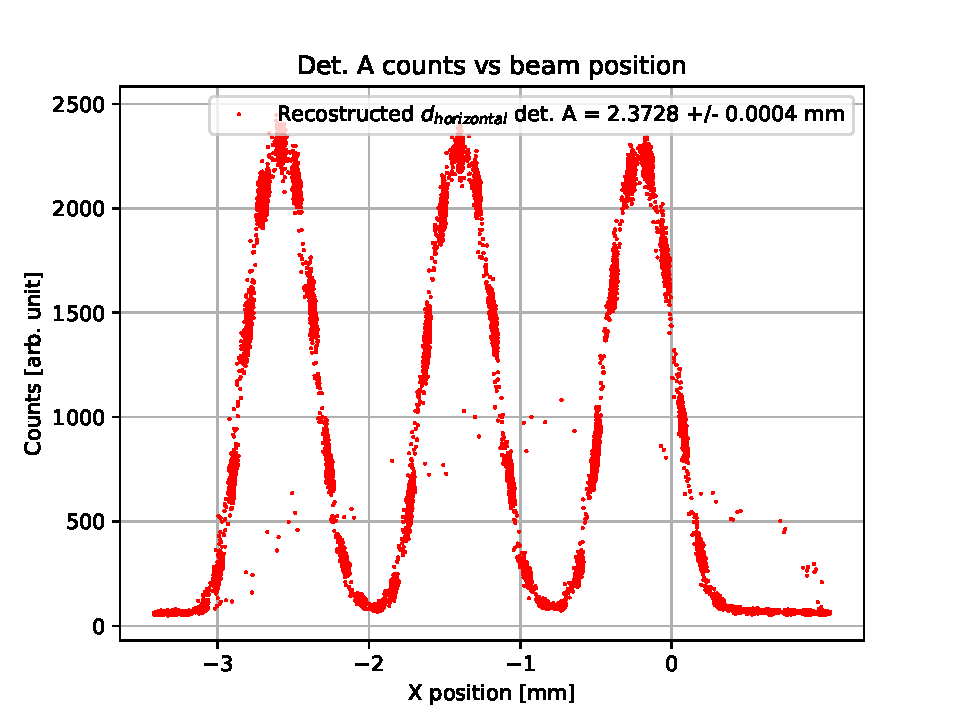
\includegraphics[width=0.45\textwidth]{Analysis/XcheckA.pdf}
\caption{Plot of the PMT Count versus the X and Y positions given in \SI{}{\milli \meter}.}
\label{fig:CheckHori}
\end{figure}

For brevity, we report only the plot for the $X$ position. The result for $Y$ are analogous.

\subsection{Current (PIMO) Calibration} \label{CurrentCalibration}

Other two calibration parameters required are about the energy and the current of the beam, and are measured with PIMO (current monitor) and ENMO (energy monitor).  In the analysis, the current is given in $\SI{}{\micro \ampere}$ and the beam energy in $\SI{}{\kilo \electronvolt}$.

The relation between the values measured in $\SI{}{\volt}$ units and the real values in $\SI{}{\micro \ampere}$ and $\SI{}{\electronvolt}$ is linear:

\begin{align*}
I(\SI{}{\micro \ampere}) = m I(\SI{}{\volt}) + q
\end{align*}

For the current monitor, the two coefficients are determined raising the beam current from $\SI{10}{\micro \ampere}$ to $\SI{22}{\micro \ampere}$ in several step. For each step we compare the nominal values of the current with the values measured in $\SI{}{\volt}$, the values are shown in figure \ref{fig:ScanCurrent}

\begin{figure}[ht]
\centering
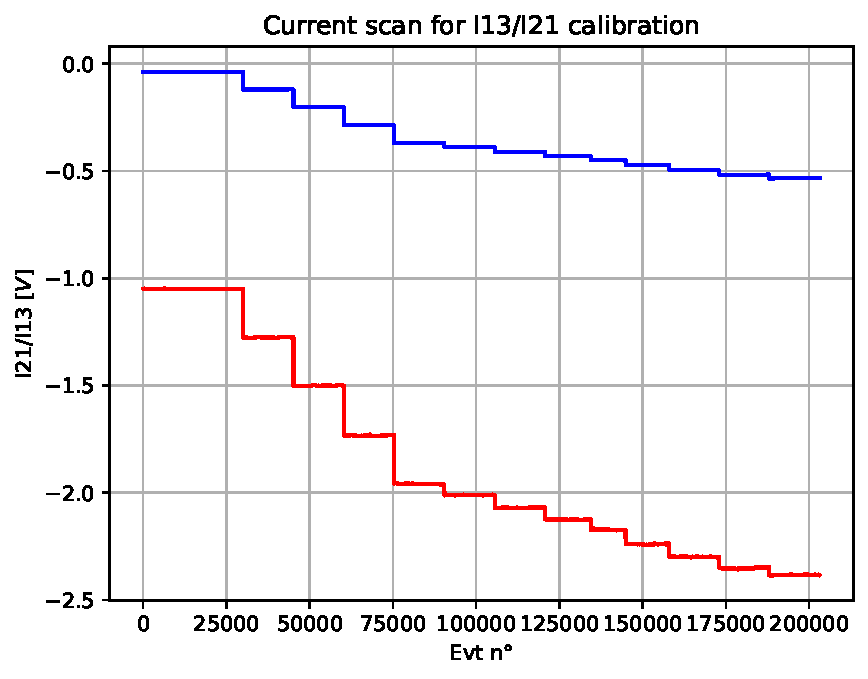
\includegraphics[width = 0.5\textwidth]{Analysis/Calibrations/ScanI21I13.pdf}
\caption{Current scan for the calibration, each step correspond to a run with a different beam current. The $x$ axis represents the number of the event analyzed, and each event is $\SI{80}{\milli \second}$ long.}
\label{fig:ScanCurrent}
\end{figure}

with a linear fit, $m$ and $q$ are determined. These parameters are added in the standard configuration file, where the analysis program loads all the coefficients needed to process the data.

\begin{figure}[hbtp]
\centering
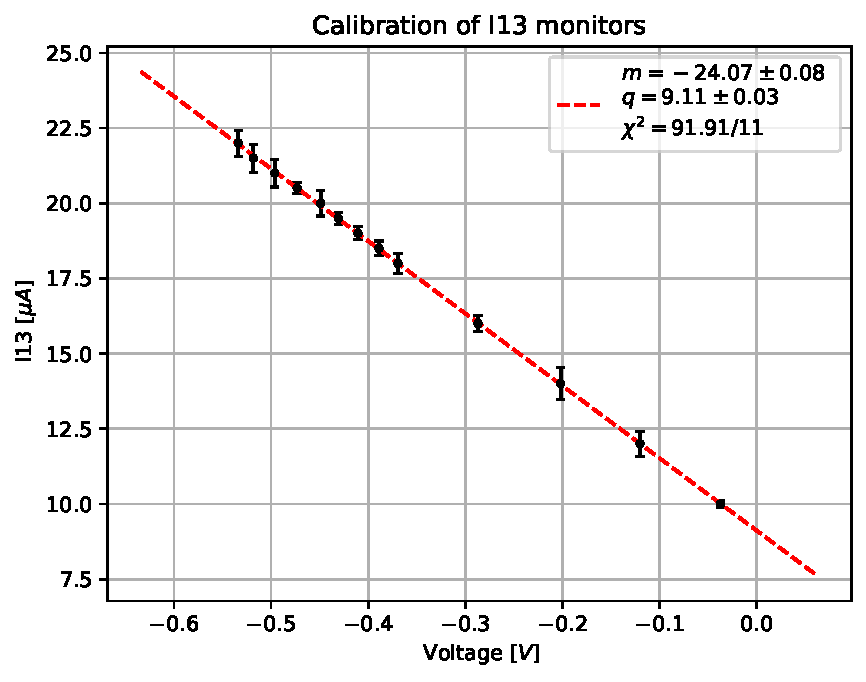
\includegraphics[width = 0.45\textwidth]{Analysis/Calibrations/I13.pdf}
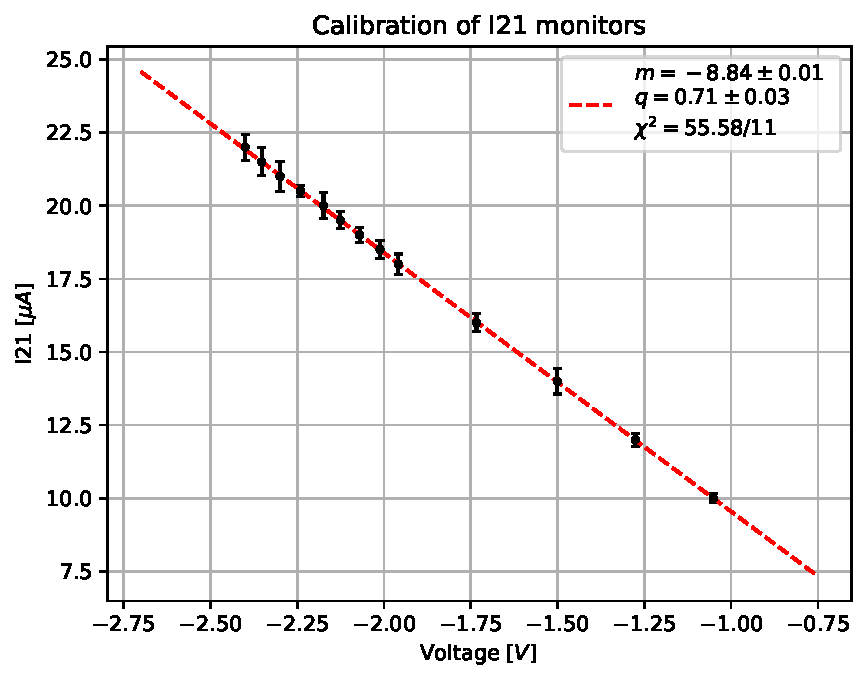
\includegraphics[width = 0.45\textwidth]{Analysis/Calibrations/I21.pdf} 
\caption{Calibrations plots for PIMO I21 and PIMO I13, the errors are multiplied by $25$.}
\label{fig:PimoCalib}
\end{figure}

The coefficients measured with the fit are shown in the figure \ref{fig:PimoCalib}. The errors shown in both the plots are given by the sampling standard deviation formula, applied to each step in plot \ref{fig:ScanCurrent}. The error $\sigma_{vfc}$ is related to uncertainty of VFCs and beam monitors, and is propagated to the $y$ axis. 
Yet, we are underestimating the error associated with the nominal beam current $I$, whose accuracy is not known. We suspect that is not negligible compared to $\sigma_{vfc}$.

\subsection{Energy Monitor (ENMO) calibration.} 

The ENMO calibration is performed in a different way from the other monitors. exploiting the polarity signal which controls the beam polarization at the source of the acceleration. The MAMI operators use the signal to create artificially a difference in the beam energy that is correlated to the beam polarization, with the last two sub-events having a higher energy with respect to the first two. The energy difference is nominally $\SI{22.6}{\kilo \electronvolt}$. Since the nominal difference is known, the scaling factor which convert from $\SI{}{\volt}$ to $\SI{}{\kilo \electronvolt}$ is easy to compute. The energy difference between the sub-events $\delta E$ (with $E_{18}$ being the energy monitor) is defined as:

\begin{equation*}
\delta E = \frac{E_{18}[2] + E_{18}[3]}{2} - \frac{E_{18}[0] + E_{18}[1]}{2} 
\end{equation*}

The measured values of $\delta E$ are shown in an histogram in figure \ref{fig:EnergyCalibration}. Three runs, collected with different currents of the beam, were collected. As the output voltage signal from the XY monitor, also the energy monitor is proportional to the current, as mentioned in equation \ref{eq:SignalToVfc}. The relation between energy $E \, \SI{}{\kilo \electronvolt}$ and the signal amplitude of the energy monitor $U \, \SI{}{\volt}$ is given by:

\begin{equation} \label{eq:EnergyVolt}
 E \, [\SI{}{\kilo \electronvolt}] = c_{E} \cdot \dfrac{ U \, [\SI{}{\volt}]}{i}
\end{equation}

So, if we invert the relation, we have that:

\begin{equation}
c_{E} = \frac{E}{U} \, \cdot i
\end{equation}  

This is the formula to compute the conversion factor for the energy monitor. The beam current was set to 0, \SI{15}{\micro \ampere} and \SI{20}{\micro \ampere}. The run with zero current is useful to check presence of an offset.

\begin{figure}[!h]
\centering
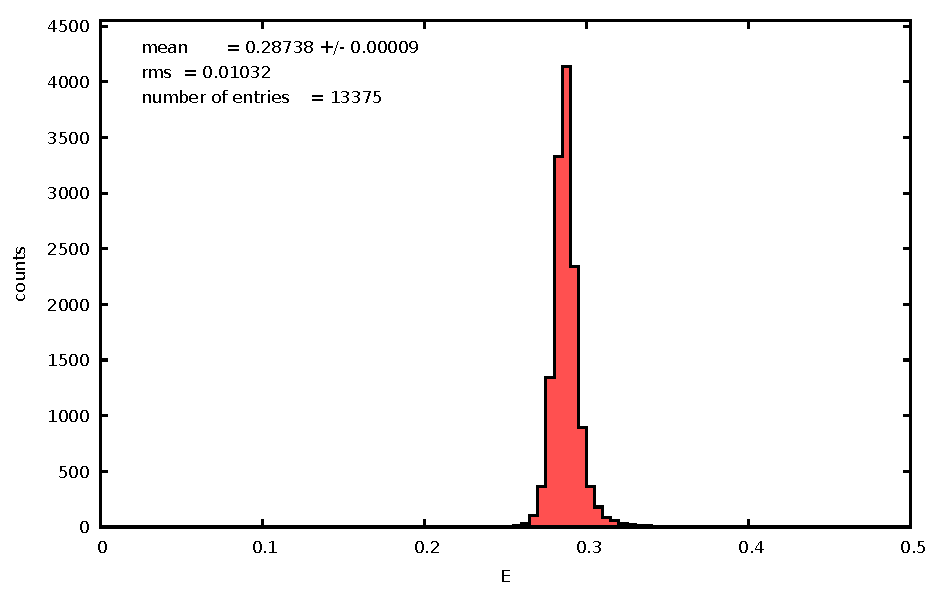
\includegraphics[width = 0.45\textwidth]{Analysis/ENMOvoltage20.pdf}
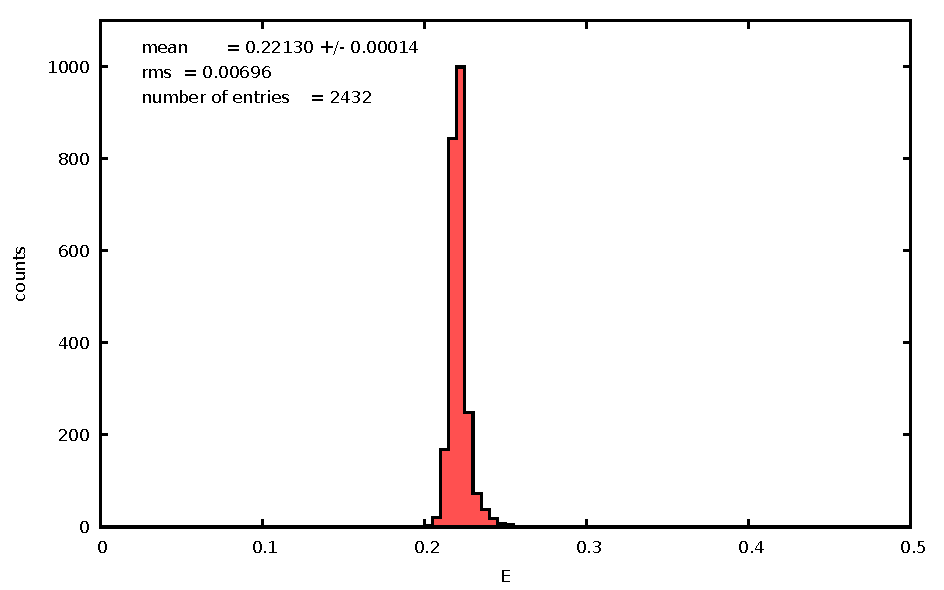
\includegraphics[width = 0.45\textwidth]{Analysis/ENMOvoltage15.pdf} 
\caption{Histograms or $\delta E$ with the beam current $\SI{20}{\micro \ampere}$ on the left and $\SI{15}{\micro \ampere}$ on the right.}
\label{fig:EnergyCalibration}
\end{figure}


To study the dependence on the current, a linear fit is done (see figure \ref{fig:EnmoFit}). The $c_{E}$ conversion parameter is obtained taking the coefficient parameter $m$ from the fit and substituting in the expression:

\begin{align*}
C_{E} =  \frac{\SI{22.6}{\kilo \electronvolt}}{m}
\end{align*}

From this we obtain the value $c_{E} = +1595.2$ necessary to convert from Voltage units to $\SI{}{\kilo \electronvolt}$.

\begin{figure}[!h]
\centering
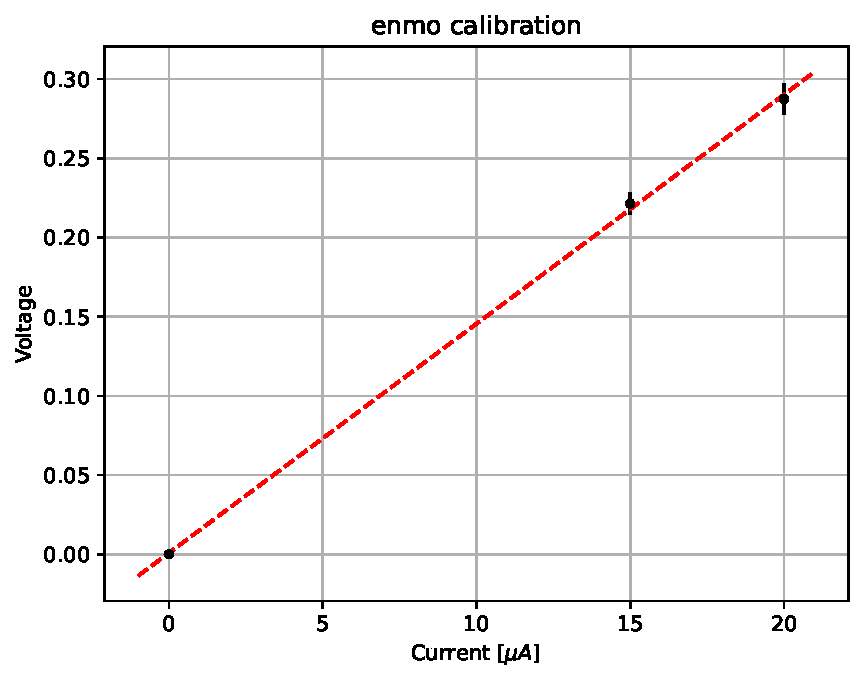
\includegraphics[width = 0.5\textwidth]{Analysis/Calibrations/E18_Calibration.pdf}
\caption{Calibration of ENMO monitor, plot of the ENMO voltage values versus the current.}
\label{fig:EnmoFit}
\end{figure}

To check the procedure, in figure \ref{fig:CheckEnmo} we plot $\delta E$ given in physical units. For \SI{15}{\micro \ampere} $\delta E = 23.519 \pm 0.014 \SI{}{\kilo \electronvolt}$ and for \SI{20}{\micro \ampere} $\delta E = 22.600 \pm 0.007 \SI{}{\kilo \electronvolt}$.

\begin{figure}[!h]
\centering
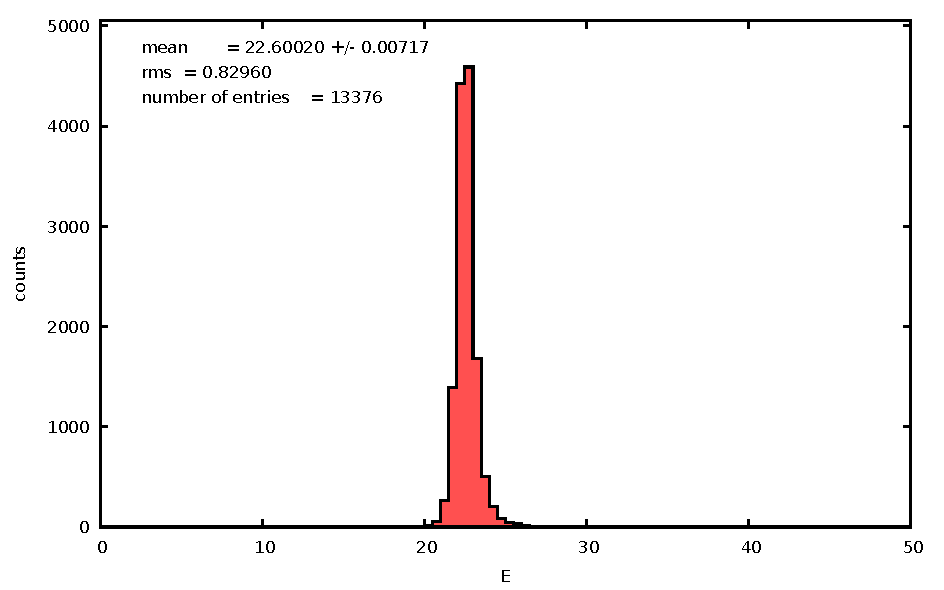
\includegraphics[width = 0.45\textwidth]{Analysis/ENMOCheck20.pdf}
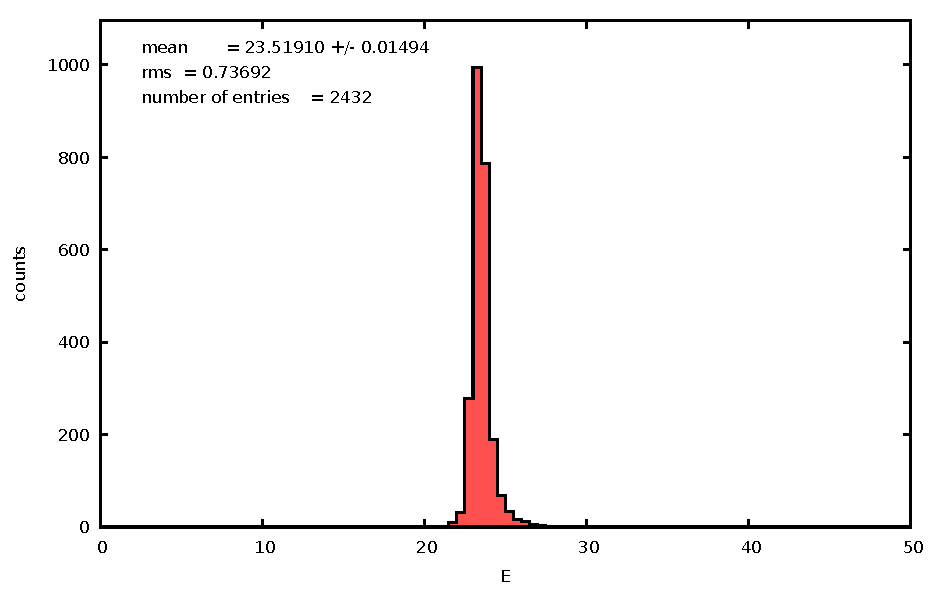
\includegraphics[width = 0.45\textwidth]{Analysis/ENMOCheck15.pdf} 
\caption{Plot for the physical quantities computed in the data tree, for two different current of the beam (on the left $\SI{20}{\micro \ampere}$, $\SI{15}{\micro \ampere}$ on the right)}
\label{fig:CheckEnmo}
\end{figure}

\newpage
\subsection{Calibration of the PMTs} \label{PMTsCalib}

Several scans in attenuation of the NINO board were performed on the beam, to choose the best working point for the PMTs of the detectors. The same procedure used in the laboratory was followed: with a beam intensity of $\SI{10}{\micro \ampere}$ we acquired data runs one minute long, varying the attenuation. 

\begin{figure}[hbtp]
\centering
\subfloat[][\emph{Attenuation scan for the PMTs of detector B} ]
{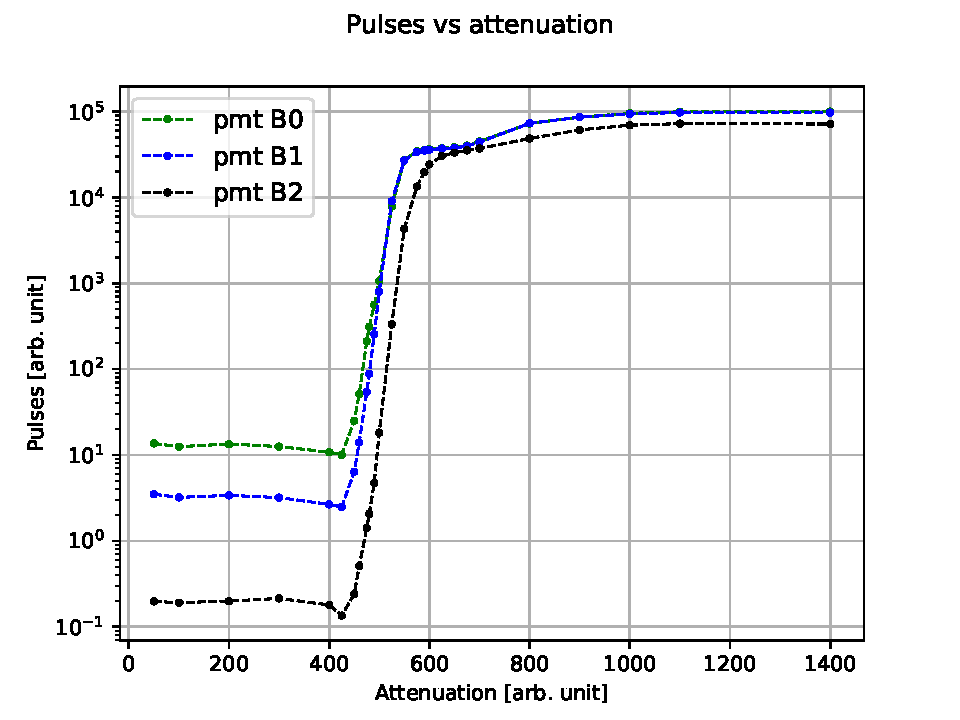
\includegraphics[width = 0.75\textwidth]{Analysis/CalibrationPMT/AttenuationScanB.pdf}}
\caption{Scan in attenuation of the NINO board, with $\SI{10}{\micro \ampere}$. Each point represents the averaged of the counts made on all sub-events of a single data run. Each data run is $\SI{1}{\minute}$ long, which correspond to $3000$ sub-events.}
\label{fig:AttScanB}
\end{figure}

\begin{figure}[hbtp]
\centering
\commento{
\subfloat[][\emph{Attenuation scan for the PMTs of detector B} ]
{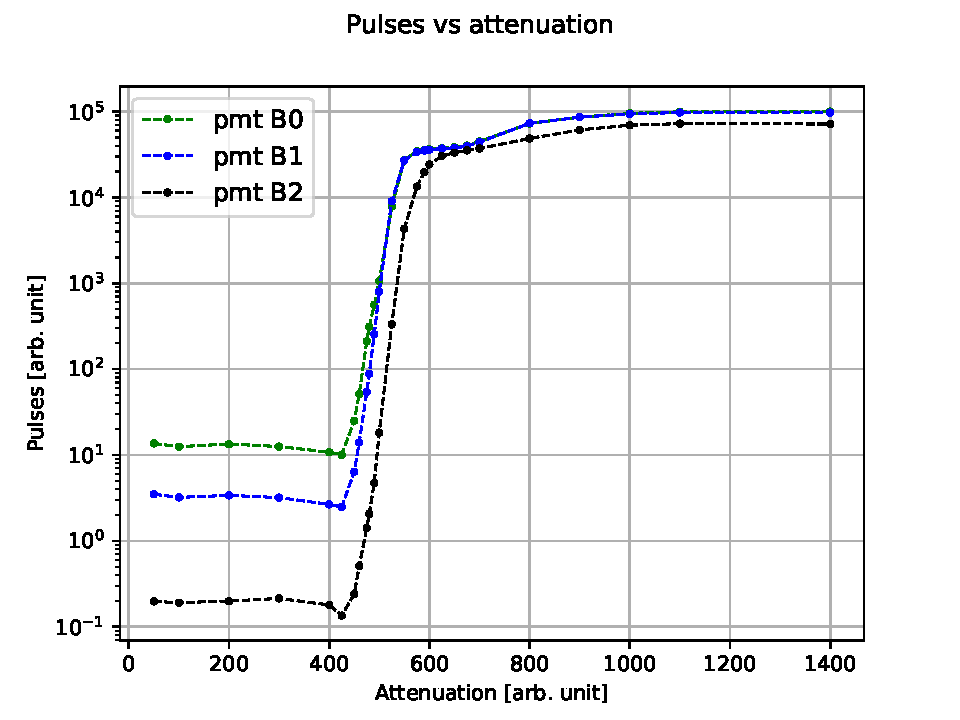
\includegraphics[width = 0.5\textwidth]{Analysis/CalibrationPMT/AttenuationScanB.pdf}} \\}
\subfloat[][\emph{Attenuation scan for the PMTs of detector B}]
{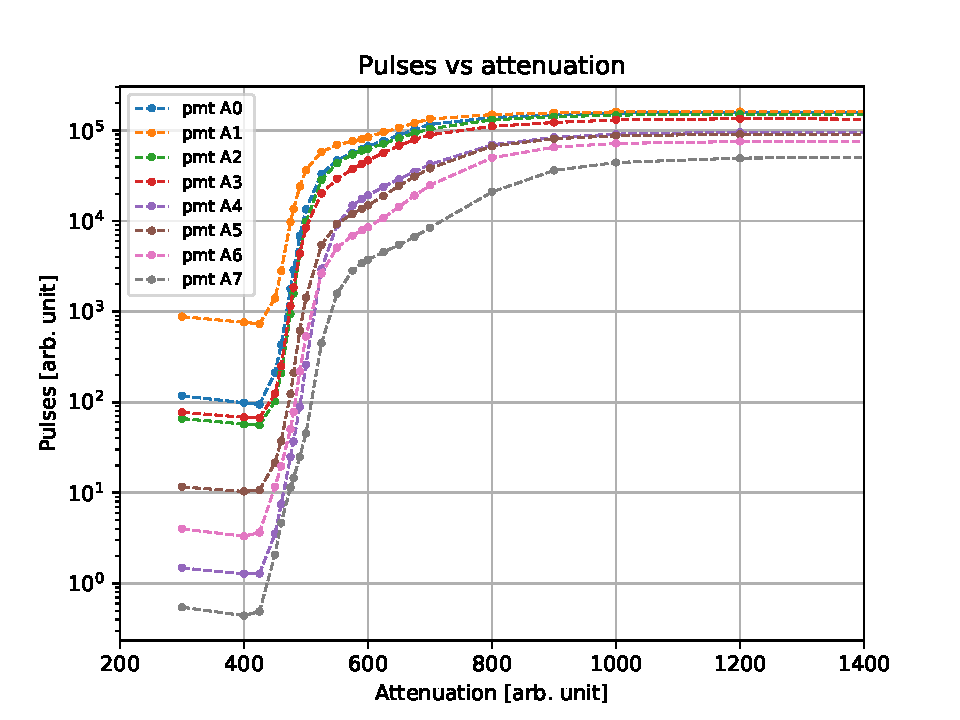
\includegraphics[width = 0.75\textwidth]{Analysis/CalibrationPMT/AttenuationScanA.pdf}}
\caption{Scan in attenuation of the NINO board, with $\SI{10}{\micro \ampere}$. Each point represents the averaged of the counts made on all sub-events of a single data run. Each data run is $\SI{1}{\minute}$ long, which correspond to $3000$ sub-events.}\label{fig:AttScan}
\end{figure}

The PMTs counts in \ref{fig:AttScan} and \ref{fig:AttScanB} are visualized in a different way. It is preferable to visualize the increment of number of signals that pass the threshold selection of NINO board. For this reason, we want to differentiate the data showed in the plots. This procedure consist in computing the difference between the counts at a certain point and the previous one, and dividing by the increment in attenuation, in equation \ref{eq:Differentiang}.

\begin{equation} \label{eq:Differentiang}
Spectra = \frac{N(att_{i}) - N(att_{i-1})}{att_{i} - att_{i-1}} 
\end{equation}

With this formula we compute $\frac{\partial N}{\partial att}$, the discrete derivative of the data shown in figure \ref{fig:AttScan}.

\begin{figure}[!hbtp]
\centering
\subfloat[][\emph{B0} ]
{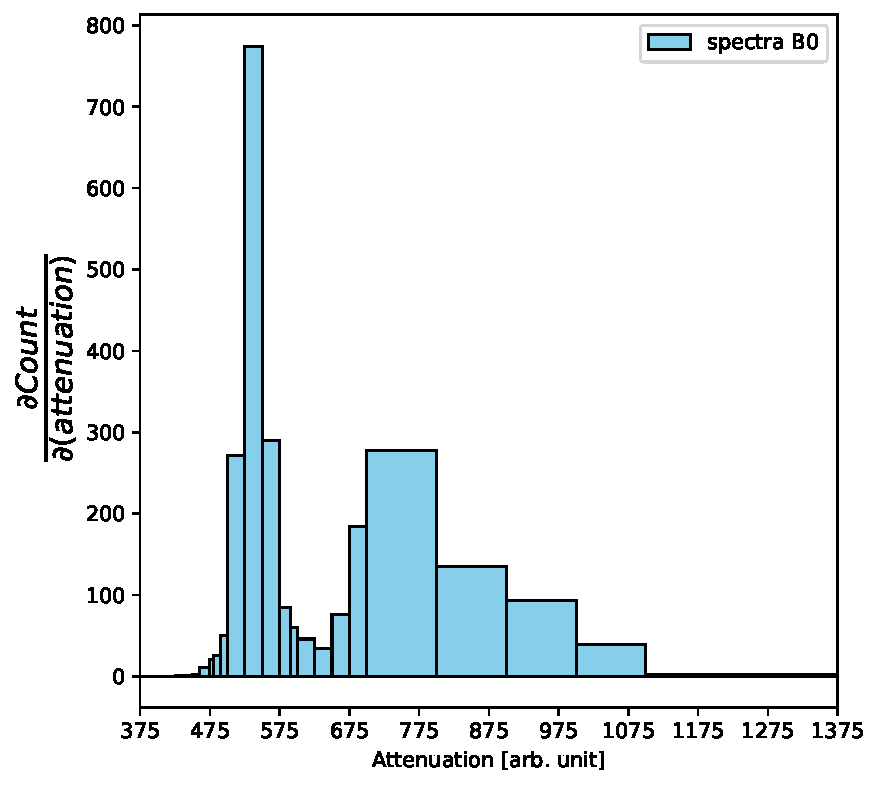
\includegraphics[scale = 0.4]{Analysis/CalibrationPMT/B0.pdf}}
\subfloat[][\emph{B1}]
{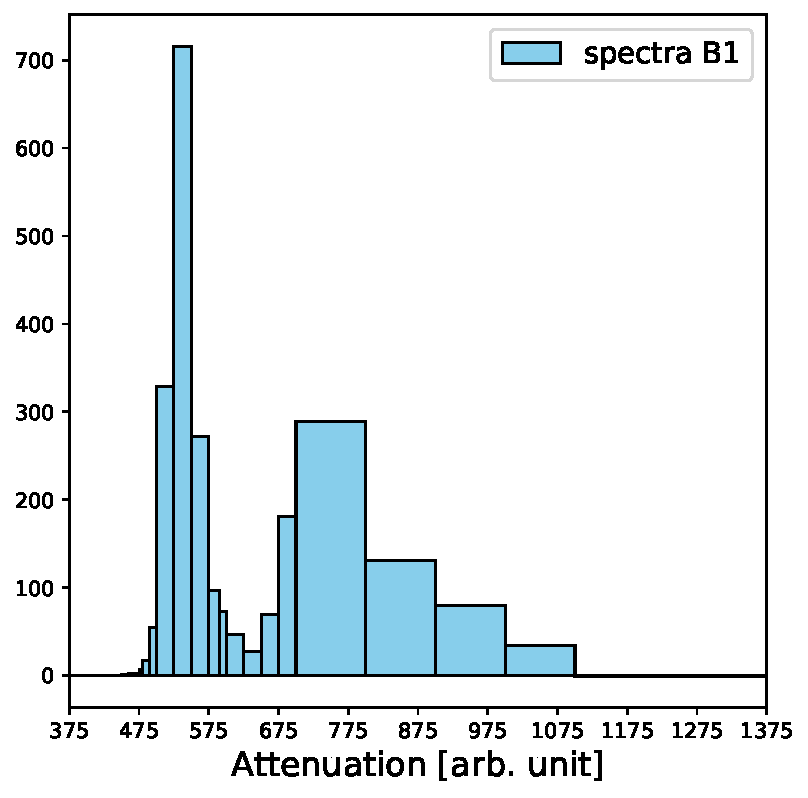
\includegraphics[scale = 0.4]{Analysis/CalibrationPMT/B1.pdf}}\\
\subfloat[][\emph{B2}]
{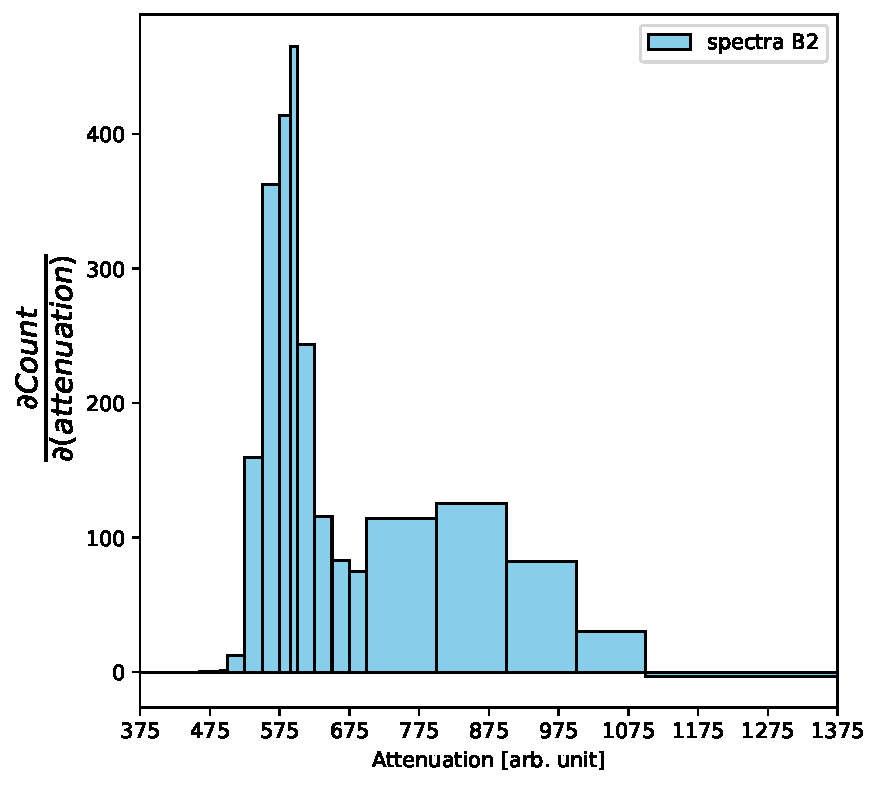
\includegraphics[scale = 0.4]{Analysis/CalibrationPMT/B2.pdf}}
\caption{Reconstructed spectra for Detector B}
\label{fig:Spectra}
\end{figure}

These plots are used to identify a good point to select the attenuation values. If we look at the plots \ref{fig:ThrvsAtt}, we can see that the physical threshold does not scale linearly with changing the \textit{Att} value, and for high values of \textit{Att}, the threshold falls quickly at zero. Looking at the signal spectra, we identify the first peak as the electron signal. The other peak (on the right), correspond to very low threshold values, and it is identified as background noise. 
We selected the values of the attenuation between the peaks of the two distributions, maximizing the signal acceptance and trying to reject the background as much as possible.
Our discussion so far is sufficient to carry out the calibration of the PMTs and take data to measure the asymmetry. However, we would like to identify the physical threshold in $\SI{}{\milli \volt}$ instead of attenuation unit. We can use the conversion function that we discussed in figure \ref{fig:ThrvsAtt}:

\begin{align*}
f(att) = \dfrac{a}{(x - b)^{3} + d}
\end{align*} 

We point out that the parameters of this function have been obtained from data that have not been acquired during this thesis work, moreover the threshold value in the program that controls the NINO board is slightly different (we always used 600, the data are taken with 750), therefore the values in volts need probably to be rescaled by some factor, but for our discussion we are interested in a raw estimation of the signal peak:
With this conversion, we show the same plots in \ref{fig:Spectra}, with the values in the x-axis in $\SI{}{\volt}$ now.

\begin{figure}[!ht]
\centering
\subfloat[][]{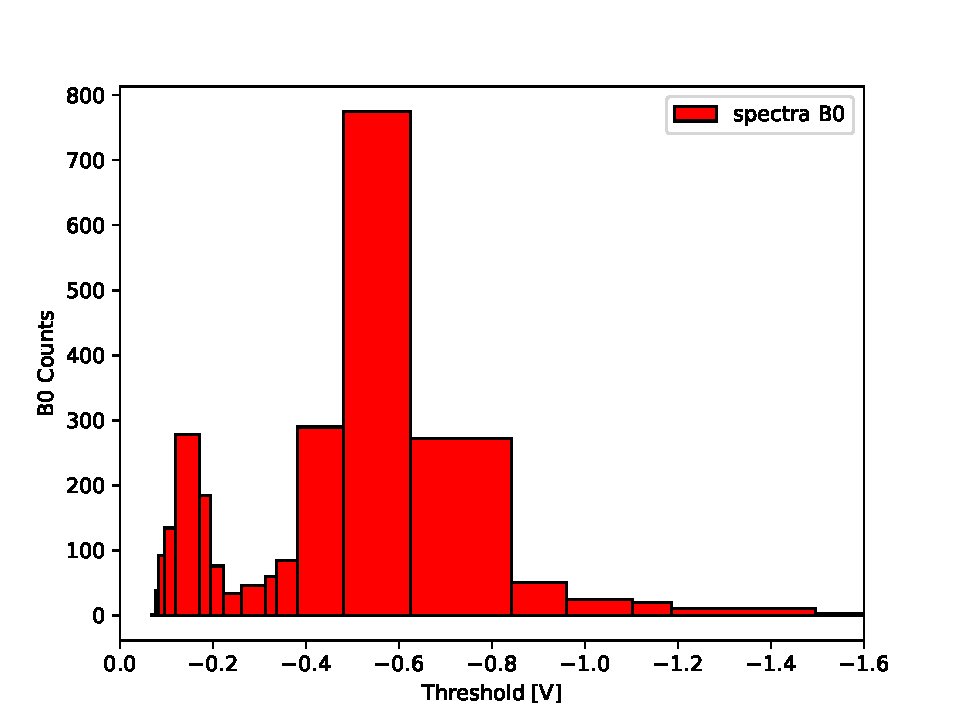
\includegraphics[width = 0.4\textwidth]{Analysis/CalibrationPMT/voltB0.pdf} }
\subfloat[][]{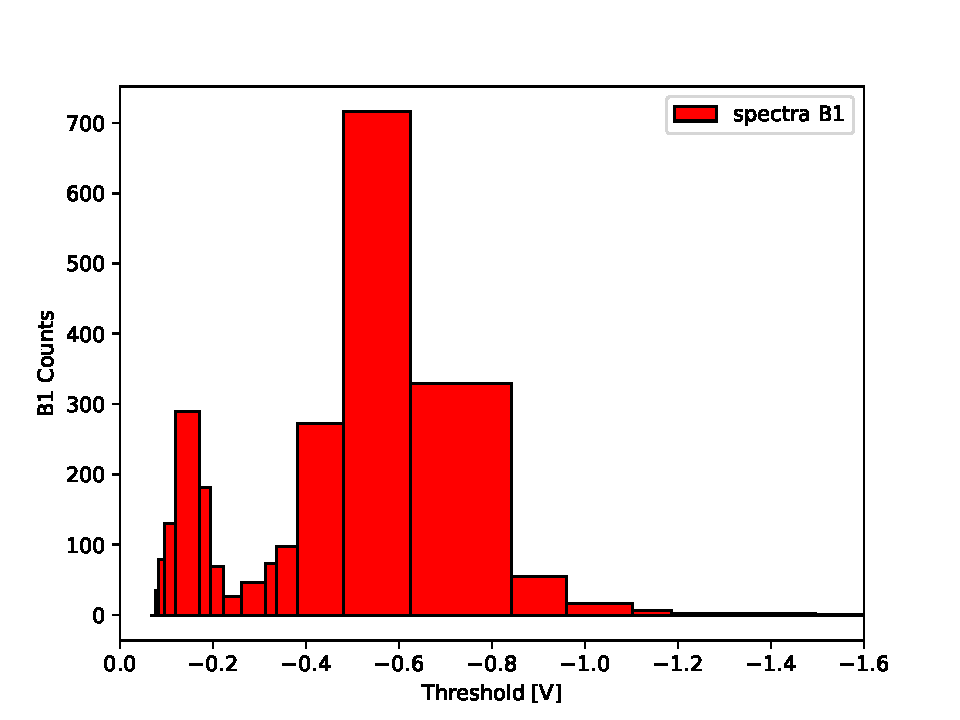
\includegraphics[width = 0.4\textwidth]{Analysis/CalibrationPMT/voltB1.pdf}}\\
\subfloat[][]{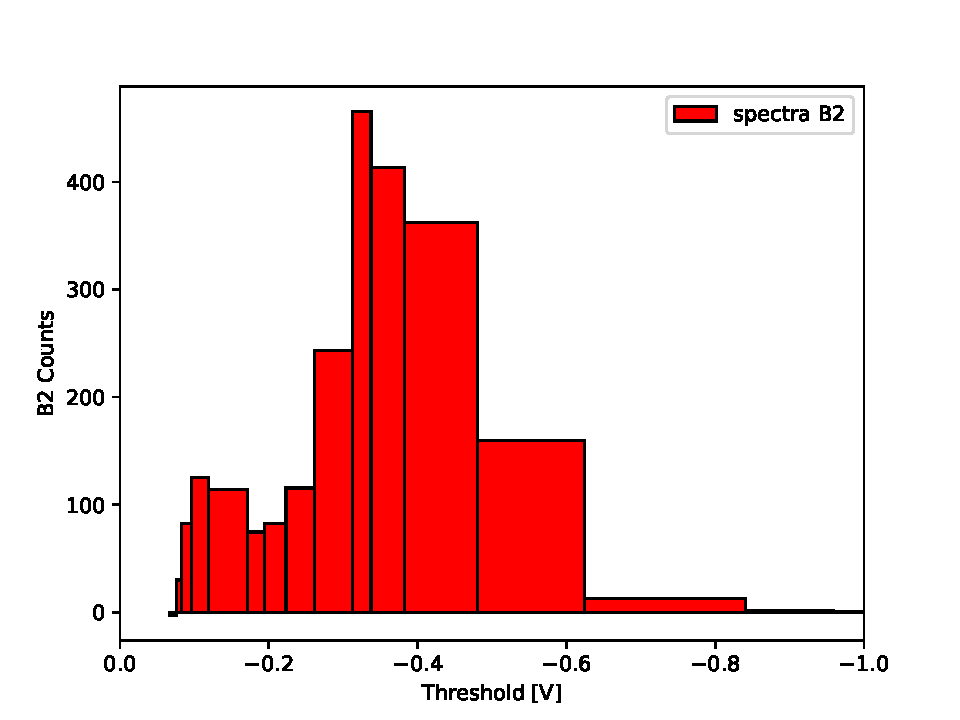
\includegraphics[width = 0.4\textwidth ]{Analysis/CalibrationPMT/voltB2.pdf}}
\end{figure}

We now see clearly two peaks, the signal and the background, that are reversed respect to figure \ref{fig:Spectra}.
We discuss now a simple model that we used to describe how the PMT Counts vary when we raise the attenuation. From the plot \ref{fig:Spectra}, we assume that the two peaks are described by two gaussian distributions. Now if we think about the the probability for a signal to pass the selection, this quantity is equal to the probability of being in below the attenuation value. Using now the fact that the probability are given by the cumulative of the gaussian distribution (probability of being in the right tail) it is straightforward to deduce:

\begin{align*}
P(signal > thr) = \, \Phi(x) = \dfrac{1 + Erf(\dfrac{x - \mu}{\sqrt{2} \sigma })}{2}
\end{align*}

Considering that we have the sum of two gaussian distribution, we end with:

\begin{equation} \label{eq:ModelAtt}
\begin{split}
N(att) = \frac{n_{1} + n_{2}}{2} + (\frac{n_{1}}{2}) Erf(\dfrac{x - \mu_{1}}{\sqrt{2} \sigma_{1} })   + (\frac{n_{2}}{2}) Erf(\dfrac{x - \mu_{2}}{\sqrt{2} \sigma_{2}}) \\
\end{split}
\end{equation}

This model is used to fit the data shown in figure \ref{fig:AttScan}. The result is shown in figure \ref{fig:BestFitAtt}, the parameters obtained from the fit are reported below:

\begin{figure}[!ht]
\centering
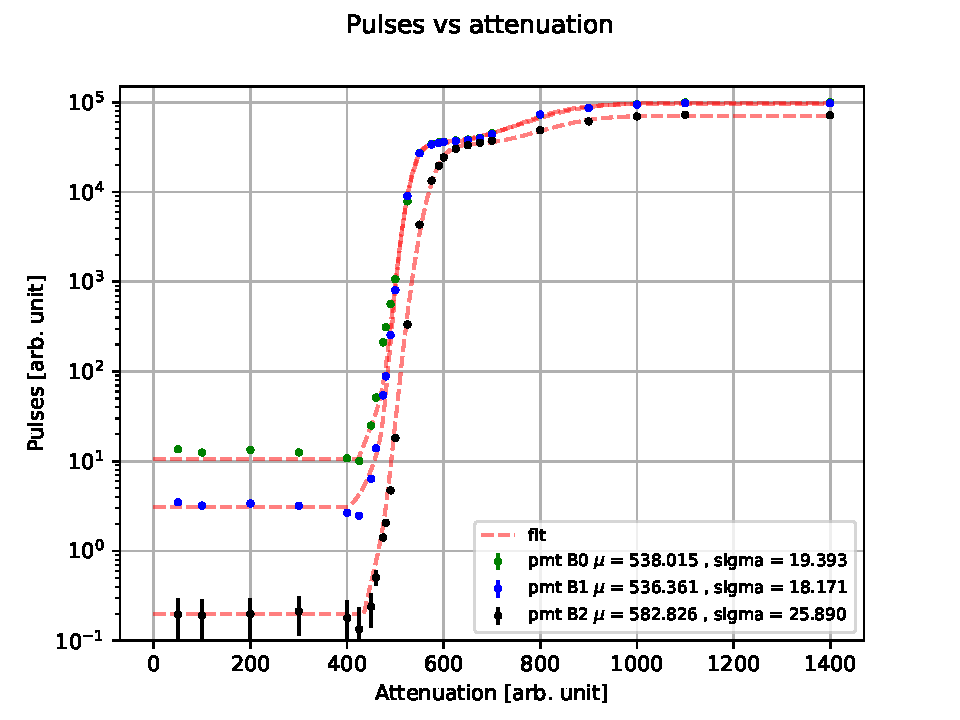
\includegraphics[width = 0.65\textwidth ]{Analysis/CalibrationPMT/Fit_attenuation.pdf}
\caption{Best fit for the data of counts versus attenuation, for detector B.}
\label{fig:BestFitAtt}
\end{figure}

\begin{table}[!ht]
\centering
\begin{tabular}{c|c|c|c|c|c|c}
\hline
 PMT   &  $\mu_{1}$         &  $\sigma_{1}$         & $\mu_{2}$          & $\sigma_{2}$   & n1                & n2                 \\
\hline
 B0    & 538.0 +/- 1.3 & 19.4 +/- 1.1 & 798 +/- 8 & 103 +/- 4 & 34277 +/- 662 & 64244 +/- 1538 \\
 B1    & 536.4 +/- 0.9 & 18.2 +/- 0.7 & 783 +/- 5 & 89 +/- 2  & 34053 +/- 475 & 61636 +/- 1109 \\
 B2    & 582.8 +/- 1.2 & 25.9 +/- 1.0 & 824 +/- 8 & 88 +/- 6  & 32880 +/- 758 & 37930 +/- 1245 \\
\hline
\end{tabular}
\caption{Best fit result for the model defined in equation \ref{eq:ModelAtt}}
\end{table}

From these result we measure the mean $\mu_{1}$ and $\mu_{2}$ for the signal and the background given in attenuation units. The correct value of attenuation is set between the two observed peaks, in order to reject the background and take only the signal coming from the scattered electrons. The same procedure was followed also for the detector A, the plots are not reported, for brevity.
With this procedure, the \textit{Att} value has been selected. The values are reported in table \ref{tab:AttSettings}

\begin{table}[ht]
\centering
\begin{tabular}{cccccccccccc}
PMT $n^{\circ}$& B0 & B1 & B2 & A0 & A1 & A2 & A3 & A4 & A5 & A6 & A7 \\
\hline
\textit{Att} & 600 & 600 & 625 & 600 & 590 & 600 & 600 & 600 & 590 & 600 & 600 \\
\end{tabular}
\caption{Attenuation settings for both the detectors.}
\label{tab:AttSettings}
\end{table}


\subsection{Auto-calibration Procedure} \label{Autocalib}

In this section we present the last calibration technique needed in the data-process. The auto-calibration is a special operation mode of the MAMI accelerator, during which the beam current is made to vary in a controlled way. Through these special runs is possible to obtain again the current scaling factor that we discussed in section \ref{CurrentCalibration} and  it is possible to study the linearity of the PMTs. During the auto-calibration, the beam current is raised from $\SI{9}{\micro \ampere}$ to $\SI{11.125}{\micro \ampere}$ in step of $\SI{0.125}{\micro \ampere}$, as shown in figure \ref{fig:Autocalibration}

\begin{figure}[!ht]
\centering
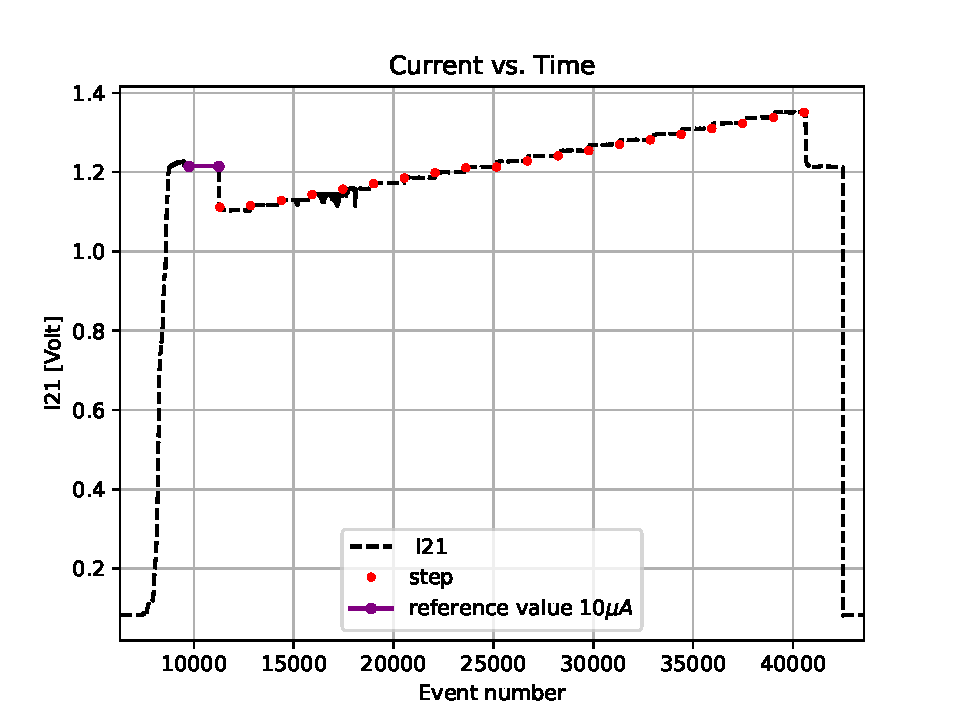
\includegraphics[width = 0.75\textwidth]{Analysis/Autocalib/Current.pdf}
\caption{Auto-calibration: in this plot we have the voltage value of I21 monitor. The current is first stabilized around $\SI{10}{\micro \ampere}$, then it is raised from $\SI{9}{\micro \ampere}$ (the step lower down) to $\SI{11.125}{\micro \ampere}$ in step of $\SI{0.125}{\micro \ampere}$.}
\label{fig:Autocalibration}
\end{figure}

 From a linear fit of the PMTs counts vs. current intensity the angular coefficient and the offset are measured. The offset is particular important because give rise of a possible systematic error that influence the final asymmetry result. It is simple to demonstrate this, if a relation of the type $N = mI + N_{0} $ holds. Consider the following quantity:

\begin{align*}
\overline{N} = \frac{N_{\uparrow} + N_{\downarrow}}{2}
\end{align*} 

we can express $N_{\uparrow}$ and $N_{\downarrow}$ in this way using the asymmetry $A_{n} = \frac{N_{\uparrow} - N_{\downarrow}}{N_{\uparrow} + N_{\downarrow}}$:

\begin{align*}
N_{\uparrow} = \overline{N} + A_{n}\overline{N} \\
N_{\downarrow} = \overline{N} - A_{n}\overline{N} 
\end{align*}

Now we suppose that $\overline{N}$ is linear dependent on the current in the way we defined above, so:

\begin{align*}
N_{\uparrow} = mI + N_{0} + A_{n}(mI) \\
N_{\downarrow} = mI + N_{0} - A_{n}(mI) 
\end{align*}

We are supposing that the offset $N_{0}$, we assume that the present offset does not contribute to the asymmetry, i.e. it is not correlated to the signal of the scattered electrons, but is due to processes of another type, therefore in the previous formulas only the $mI$ counts must be multiplied by the asymmetry $A_{n}$. Therefore if we substitute everything in the definition of the transverse asymmetry:

\begin{equation} \label{eq:Systematic}
A^{'} = \dfrac{N_{\uparrow} - N{\downarrow}}{N_{\uparrow} + N{\downarrow}} = \dfrac{A_{n} (2mI)}{ (2mI) + 2N_{0} } = A_{n} \dfrac{1}{1 + \frac{N_{0}}{mI}} = A_{n}\cdot c
\end{equation} 

In the last passage we learn that the presence of an offset can decrease the reconstructed asymmetry. So it is important to determine quantitatively $N_{0}$ and $m$ in order to be able to correct for this effect. The strategy used is quite simple: every three hours of production data, we asked MAMI to start the auto-calibration program. With all the auto-calibration runs, we estimate $N_{0}$ for each PMT, separately. Then all this quantities are saved in a file so that the analysis program can retrieve the parameters and subtract them from the PMT counts.
In this way every three hours the PMT are corrected, taking care also of the possibility that the the linearity of the PMTs can change after hours of use of the PMTs (for example it can decrease the efficiency). With a linear fit we can estimate the angular scale coefficient and the offset to convert from I21 voltage values to physical values of the current. The procedure in repeated for the $8$ auto-calibration acquisition we had during the beam time, so we can also take care of possible time variations.

\begin{figure}[!hbtp]
\centering
\subfloat[][\emph{Current scan for detector A, the error are multiplied by a factor of $20$.}]{
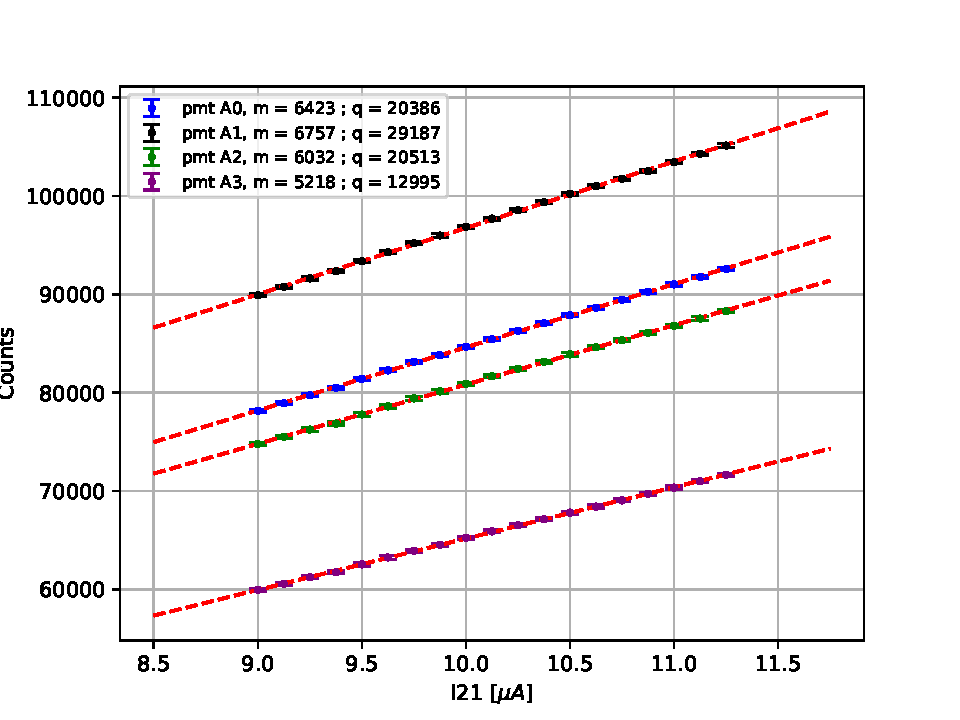
\includegraphics[width = 0.49\textwidth]{Analysis/Autocalib/fitA0-3.pdf}}
\subfloat[][\emph{Current scan for detector A, the error are multiplied by a factor of $20$.}]{
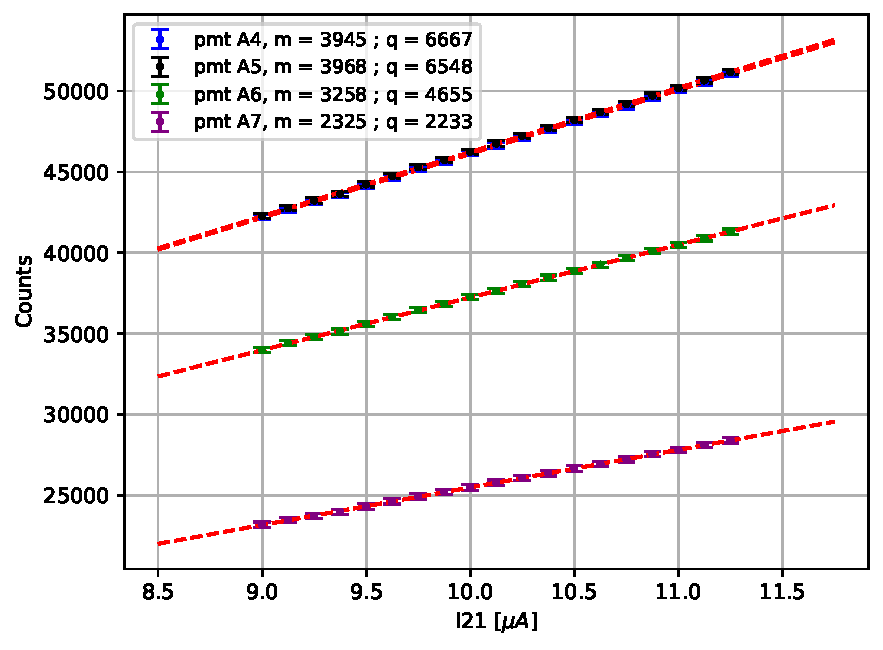
\includegraphics[width = 0.49\textwidth]{Analysis/Autocalib/fitA4-7.pdf}}
\caption{PMT Rates vs current (from I21 monitor), linear model is used to fit the data.} 
\label{fig:AutocalibFit}
\end{figure}

\begin{figure}[!hbtp]
\centering
\subfloat[][\emph{Current scan for detector B, the error are multiplied by a factor of $20$.}]{
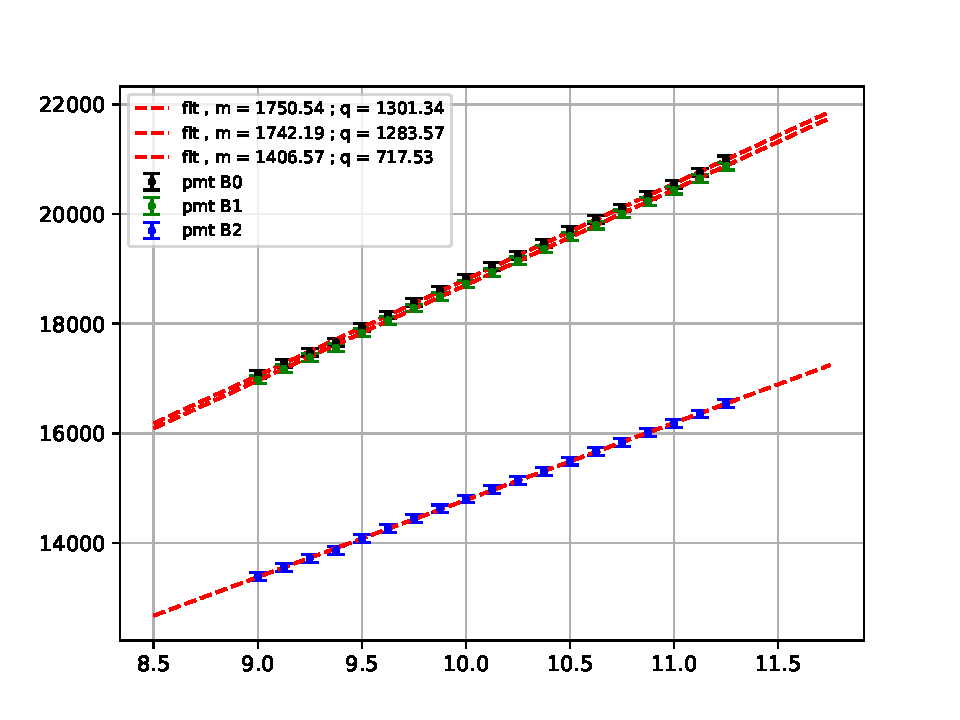
\includegraphics[width = 0.5\textwidth]{Analysis/Autocalib/fitB.pdf}} \\
\caption{PMT Rates vs current (from I21 monitor), linear model is used to fit the data.} 
\label{fig:AutoBcalibFit}
\end{figure}

The figures shown in \ref{fig:AutocalibFit} and \ref{fig:AutoBcalibFit} are referred to the data acquired for the first auto-calibration run; the values of slope and offset measured during the first auto-calibration are in table \ref{tab:PMToffset}. These data are valuable because we can compute $c$, the factor that appears in equation \ref{eq:Systematic}:
\begin{table}[!h]
\centering
\begin{tabular}{c|c|c|c}
\hline
 PMT & m [$\SI{}{\micro \ampere}^{-1}$] & Offset & c  \\
\hline
 B0  & 1750 &  1301 &  0.930 $\pm$ 0.003\\
 B1  & 1742 &  1283 &  0.931 $\pm$ 0.003\\
 B2  & 1406 &   717 &  0.951 $\pm$ 0.003\\
 A0  & 6423 & 20385 &  0.759 $\pm$ 0.002\\
 A1  & 6756 & 29187 &  0.698 $\pm$ 0.003\\
 A2  & 6032 & 20513 &  0.746 $\pm$ 0.002\\
 A3  & 5218 & 12995 &  0.800 $\pm$ 0.002\\
 A4  & 3945 &  6666 &  0.855 $\pm$ 0.002\\
 A5  & 3967 &  6547 &  0.858 $\pm$ 0.002\\
 A6  & 3258 &  4655 &  0.874 $\pm$ 0.002\\
 A7  & 2325 &  2233 &  0.912 $\pm$ 0.002\\
\hline
\end{tabular}
\caption{Angular coefficient and offset obtained for the auto-calibration. The third column is contains the estimation of $c$, as defined in equation \ref{eq:Systematic}}
\label{tab:PMToffset}
\end{table}

Ignoring the presence of the offset leads to two consequences: the reconstructed asymmetry is lower, on average $ \simeq 10\%$ less than expected, and the counts are overestimated. Because the error depend on the PMT counts, as seen in equation \ref{eq:Error}, this two effect combined add up and decrease the accuracy of the asymmetry measurement
The value $c$ reported in the chapter \ref{result} can be compared with $c$ in table \ref{result}, computed as the ratio between $\frac{A_{not corr}}{A_{corr}}$, where $A_{not corr}$ stands for the asymmetry result not corrected for the offset and $A_{corr}$ are the result with offset corrected. 

\section{Data Tree Implementation}

We now discuss briefly the structure of the data that is implemented in the analysis program, important to clarify how data analysis will be developed.
The base class that is implemented in the analysis program is the \textit{Event} class. As we mention above in section \ref{FirstDescription}, we do not intend to keep track of the single scattered electron, instead we analyze time series of $\SI{80}{\milli \second}$, in which we simply count all the electrons detected in this time interval. The work-flow of the analysis program is load the binary file collected during the beam time, parsing  one event at a time and processing the raw-data from the beam monitors and the detectors (see figure \ref{fig:DataFlow}). 

\begin{figure}[!hbtp]
\centering
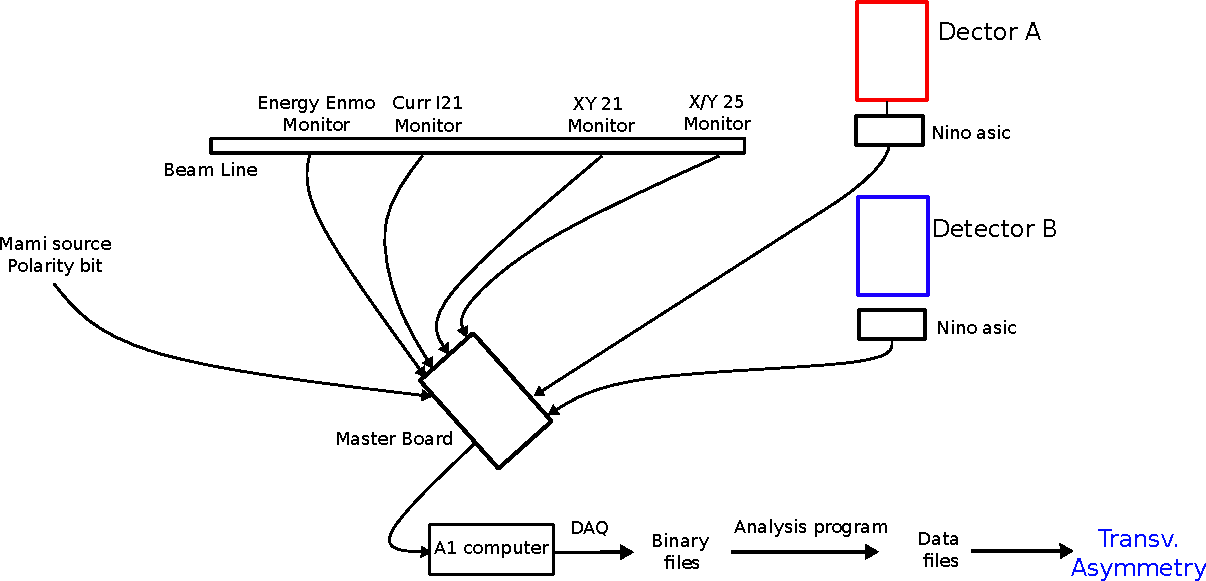
\includegraphics[width = 0.75\textwidth]{Analysis/Electronic_scheme.pdf}
\caption{Scheme of the data flow.}
\label{fig:DataFlow}
\end{figure}

During the execution of the program data files in \textit{.txt} are generated and filled with the processed data ready. The output data-file can be analyzed with any software package, such as root or python, to get the value of the asymmetry $A_{n}$. 
Referring to the figure \ref{fig:EventStructure}, we remind that every event is divided into $4$ sub-events. For each different sub-event a precise state of the polarization is defined, $+1$ for $S = \uparrow$ and $-1$ for $S = \downarrow$. Every sub-event is $\SI{20}{\milli \second}$ long; during this time interval master-board receives all the data coming from the monitors and the detectors and sent them to the data-acquisition program (DAQ) that produces the binary-files, which are the input of the main analysis program. It is important to note that for each sub-event, a single measurement is acquired from the beam monitors, which is intended as a time average of the various signals on the 20 milliseconds of sub-event duration. The sampling rate is then equal to $\SI{50}{\hertz}$.
This structure of the data is quite specific. The main reason for this setup is connected with the need to avoid as much as possible that the variations of intensity, position and energy of the beams induce an effect that add to $A_{n}$. Considering only small time series, it is assumed that the beam is quite stable, in order to reduce undesired effects.
Nevertheless, the contribution of these effects, which are indicated for brevity as false asymmetries, is considered in the final model.
Several values are saved with the number of scattered electrons, for each event. The general structure of the data tree, with the important quantities, is reported here figure \ref{fig:DataTree}

\begin{figure}[!hbtp]
\centering
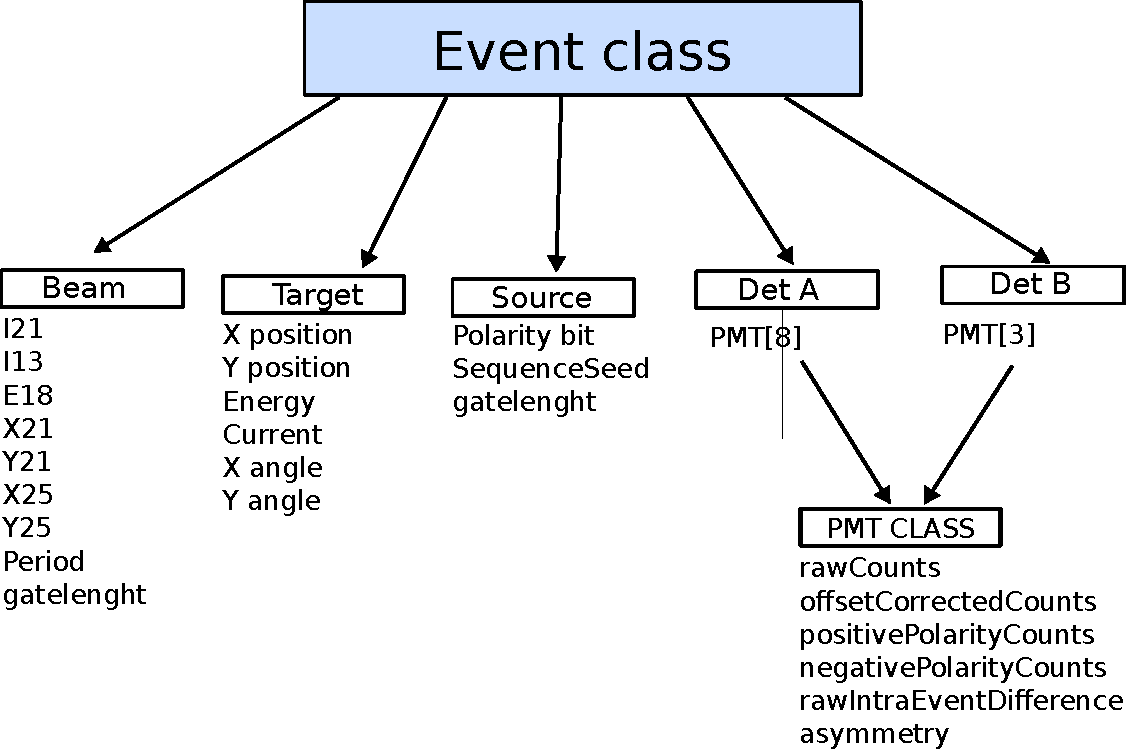
\includegraphics[width = 0.6\textwidth]{Analysis/EventClass.pdf}
\caption{Scheme of the Event class, the structure of the data tree is explained in the appendix.}
\label{fig:DataTree}
\end{figure}

The analysis program reads the binaries files, converts from binary to decimal values and computes the beam parameters from the raw data of the monitors, filling the data tree shown in the figure. We have 5 different classes, that are contained in the main \textit{Event} class. The asymmetry values are stored in the two separated classes, \textit{Det A} and \textit{Det B}. The analysis program read and analyze one event at a time, can produce also histograms for a fast visualization of the data, and generates the final output files in \textit{txt} format for the data analysis.  

\chapter{Asymmetry on Carbon and Rates on Lead Target.}

\paragraph{}
Once the calibrations are completed, the data are analyzed, to determine the transverse asymmetry on $^{12}C$. In this chapter we outline the steps involved in pre-selecting the data and in analyzing the asymmetry of the two detectors. The amount of data collected during the experiment is 23 hours of beam time, which corresponds roughly to 1 million of events.

A section is dedicated to the measurement with lead target; through these measurement, we calculate the amount of statistics needed to measure the transverse asymmetry on $Pb$ with an accuracy of $ \simeq 1/\ \, ppm$. Finally, we discuss the problem of the false asymmetries, that could influence the final result, trying to calculate their contribution directly. 
 
\section{Model for Fitting the Data} \label{Model}

One of the problems of the measurement is to take into consideration the various contributions that can change the value of the asymmetry measured by the experimental apparatus. The PMTs counts, and consequently the measured asymmetries, can be affected by the variation of the beam parameters during the time. These effects are summarized in the list below:
\begin{itemize}
\item variation of the $(x,y)$ impact position of the beam on the target
\item the variations of the incident angles $\theta_{x}$and $\theta_{y}$ on the target.
\item the uncertainty associated with the energy of the beam, a change in the energy associated with the polarization of the beam leads to different rates for the cross section.
\item the uncertainty associated with the current of the beam, in particular a difference in the 
efficiency of the source in producing electrons polarized in the two opposite directions.
\end{itemize}

All these quantities, which we will indicate in general with $\delta q$, could be correlated to false asymmetries, which influence the measured values of $A_{n}$. Furthermore, $A_{n}$ is expected to be small, in the order of ten part per million, and and beam variations can not be neglected. Correcting directly the false asymmetries that arise from these uncertainties is a difficult task, and it is easier to adopt a different strategy rather than the analytical/numerical calculation of each of them. Knowing that the beam parameters produced by MAMI are quite stable over the time, we can assume that the measured asymmetry are well described by a linear model as the following:

\begin{equation}
A_{tot} = A_{physical} \cdot P + \delta_{I} + A_{x} \delta x + A_{y} \delta y + A_{\theta_{x}} \delta \theta_{x} + A_{\theta_{y}} \delta \theta_{y}+ A_{E} \delta E 
\end{equation}

$A_{physical}$ is the aim of the experiment, $A_{x}$ and $A_{y}$ are the coefficients induced by the variation of the position of the beam, $A_{\theta_{x}}$ and $A_{\theta_{y}}$ are the coefficients associated to angles, $A_{E}$ is the coefficients associated to the beam energy and P is the polarization percentage. 
This is a first order approximation, which is valid for small variation of the beam parameters ($\delta x, \delta y, \delta \theta_{x}, \delta \theta_{y}, \delta_{E}$).
We must clarify now what we mean with $\delta x, \delta y, \delta \theta_{x}, \delta \theta_{y}, \delta_{E}$. Recalling the event structure, that we discussed in section \ref{FirstDescription}, we have a sequence of 4 different sub-events, with a polarization pattern that is randomly selected between $\uparrow,\downarrow,\downarrow, \uparrow$ and $\downarrow,\uparrow,\uparrow,\downarrow$. During the $\SI{20}{\milli \second}$ of time length of each sub-event, the beam monitors provide a single measurement of the beam parameters, and the data are saved in the data tree. The task of the analysis program is to use this raw data to calculate the relevant parameters for the analysis. Because we are working with asymmetries, the absolute values of the parameters listed above is not relevant, instead what is relevant are the differences between different polarization states of the beam. Assuming this, $\delta x, \delta y, \delta \theta_{x}, \delta \theta_{y}, \delta_{E}$ are defined by equation \ref{eq:BeamParameter}:

\begin{equation} \label{eq:BeamParameter}
\begin{split}
\delta {x} & = \Bigl(\dfrac{x_{\uparrow}(1) + x_{\uparrow}(2)}{2}\Bigl)  - \Bigl(\dfrac{x_{\downarrow}(1) + x_{\downarrow}(2)}{2}\Bigl)\\
\delta {y} & = \Bigl(\dfrac{y_{\uparrow}(1) + y_{\uparrow}(2)}{2}\Bigl)  - \Bigl(\dfrac{y_{\downarrow}(1) + y_{\downarrow}(2)}{2}\Bigl)\\
\delta {E} & = \Bigl(\dfrac{E_{\uparrow}(1) + E_{\uparrow}(2)}{2}\Bigl)  - \Bigl(\dfrac{E_{\downarrow}(1) + E_{\downarrow}(2)}{2}\Bigl)\\
\delta {\theta_{x}} & = \Bigl( \dfrac{\theta_{x,\uparrow}(1) + \theta_{x,\uparrow}(2)}{2} \Bigl) - \Bigl(\dfrac{\theta_{x,\downarrow}(1) + \theta_{x,\downarrow}(2)}{2} \Bigl)\\
\delta {\theta_{y}} & = \Bigl( \dfrac{\theta_{y,\uparrow}(1) + \theta_{y,\uparrow}(2)}{2} \Bigl) - \Bigl(\dfrac{\theta_{y,\downarrow}(1) + \theta_{y,\downarrow}(2)}{2} \Bigl)\\ 
\delta I &= \dfrac{I_{\uparrow} - I_{\downarrow}}{I_{\uparrow} + I_{\downarrow}} \\
\end{split}
\end{equation}

Each $\delta q$ represents the variation of one of the parameters of the beam within an event, so.
One may wonder why the model doesn't contain a parameter $A_{I}$ to describe the false asymmetry due to the current. We can show theoretically that the values of $A_{I}$ is equal to $1$. Starting from the definition of rate $\Gamma$:

\begin{equation} \label{eq:RatesTheoretical}
\Gamma = \frac{dN}{dt} = \frac{I_{0}}{e} \, \sigma \, \frac{n_{t} V_t}{S}
\end{equation}

where $I_{0}$ is the beam current, $e$ is the elementary charge, $n_{t}$ is the number density of the target, $V_{t}$ the target volume and S is the surface of the beam. Using \ref{eq:RatesTheoretical}, the total asymmetry $A$ is given by the equation \ref{eq:CurrentAsym}.

\begin{equation} \label{eq:CurrentAsym}
A = \dfrac{\frac{dN_{\uparrow}}{dt} - \frac{dN_{\downarrow}}{dt}}{\frac{dN_{\uparrow}}{dt} + \frac{dN_{\downarrow}}{dt}} = \dfrac{\sigma_{\uparrow} I_{0 \uparrow} - \sigma_{\downarrow} I_{0 \downarrow}}{\sigma_{\uparrow} I_{0 \uparrow} + \sigma_{\downarrow} I_{0 \downarrow}}
\end{equation}

Let's suppose now that the false asymmetry associated to the current is given by $A = A_{I} \cdot \delta I$.  
Now, the formula in the model is slightly different

\begin{equation}
A = \dfrac{\sigma_{\uparrow} - \sigma_{\downarrow}}{\sigma_{\uparrow} + \sigma_{\downarrow}} + \dfrac{I_{\uparrow} - I_{\downarrow}}{I_{\uparrow} + I_{\downarrow}} = \dfrac{2(\sigma_{\uparrow} I_{0 \uparrow} - \sigma_{\downarrow} I_{0 \downarrow})}{ 2\sigma_{\uparrow} I_{0 \uparrow} + 2\sigma_{\downarrow} I_{0 \downarrow} + \sigma_{\uparrow} I_{0 \downarrow} + \sigma_{\downarrow} I_{0 \uparrow}  }
\end{equation}

Now, the asymmetry in the cross section in expected to be of the order of $10^{-6}$. 
If we approximate $\sigma_{\uparrow} \simeq \sigma_{\downarrow}$, the two formula above are equal. In the end we have the equation \ref{eq:CurrentAsym2}.

\begin{equation} \label{eq:CurrentAsym2}
A_{tot} = A_{n} + \dfrac{I_{0 \uparrow} - I_{0 \downarrow}}{I_{0 \uparrow} + I_{0 \downarrow}} = A_{n} + \delta_{I}
\end{equation}

This is a direct consequence of the fact that the luminosity is proportional to the beam current, so we don't need to add a new parameter to the model.

\section{Data Pre-selection and Fit}

After all the calibration are performed, the analysis program is ready to produce the data-files suitable to analyze the asymmetry data for Carbon. Before proceeding with the linear fit, however, it is necessary to visualize the data to check that there are no anomalous behaviors. In fact the data can contain moments of loss of the beam current and sudden interruptions, loss of the beam polarization and even setting errors by MAMI operators can affect the experiment. Carbon data were taken from November 2nd to 4th, and consist of $28$ runs, each $1$ hour long.
The first step is to observe the PMT counts and the current trend, in order to be able to identify sudden interruptions of the beam, outliers and to check the behaviour. In figure \ref{fig::CountTrend} we show the trend over time for the of series runs.

\begin{figure}[hbtp]
\centering
\subfloat[][\emph{Counts vs. time}]{
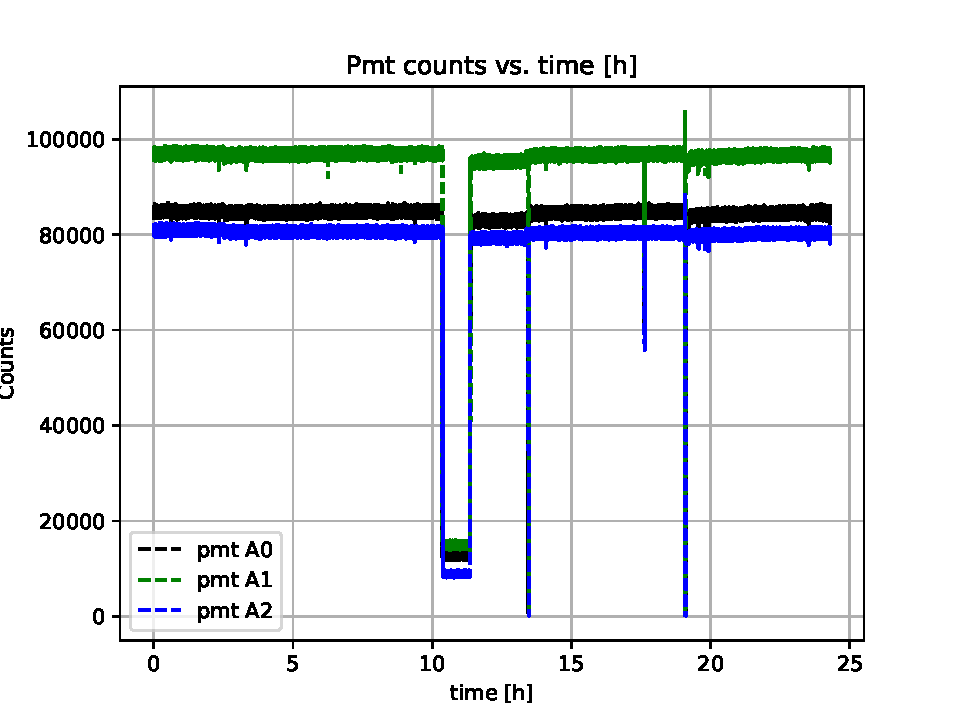
\includegraphics[width = 0.45\textwidth]{Analysis/Dataselection/BeamExample.pdf}}
\subfloat[][\emph{Asymmetry trend for PMT A0}]{
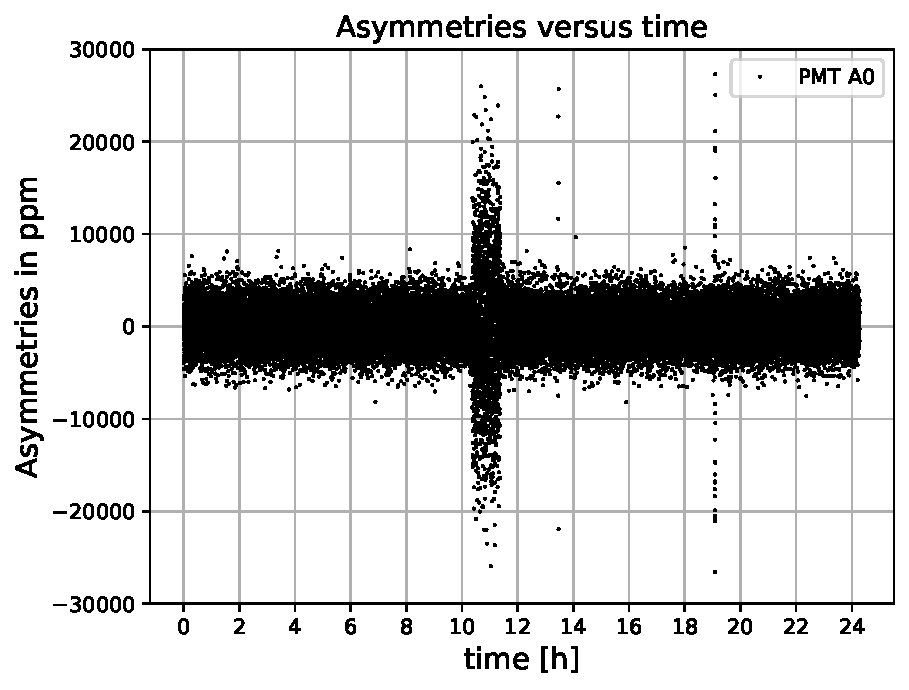
\includegraphics[width = 0.45\textwidth]{Analysis/Dataselection/AsymmetryTrend.pdf}}
\caption{On the left, counts versus time for all the runs acquired during the beam time. On the right the measured asymmetry versus time. The conversion from event number to time is made knowing that each event correspond to $\SI{80}{\milli \second}$. A total of 22 hours of beam was collected.}
\label{fig::CountTrend}
\end{figure}

This plot show that after 10 h of data acquisition the PMT counts (see plot (a) in figure \ref{fig::CountTrend}) dropped rapidly. For the beam current there is not a corresponding decrease in beam intensity. Also the $x,y$ position (\ref{fig::PositionTrend}) and the energy monitor of the beam do not show unexpected behavior, so we reject the possibility that the beam was not properly aligned to the target.
For all the PMTs of this suspecious data run, the counts are equal to the offsets measured with the auto-calibration run. 
This indicates that there was a failure in the data acquisition program, which controls the NINO board. These data are rejected completely from the analysis.
In plot \ref{fig::CountTrend} we observe abrupt variations of the asymmetry at $13.5 h$ and $19 h$, while other variations are less appreciable. These data correspond to loss of the beam intensity for a short periods of time, and are rejected as outliers. 

\begin{figure}[hbtp]
\centering
\subfloat[][\emph{Current trend over time.}]{
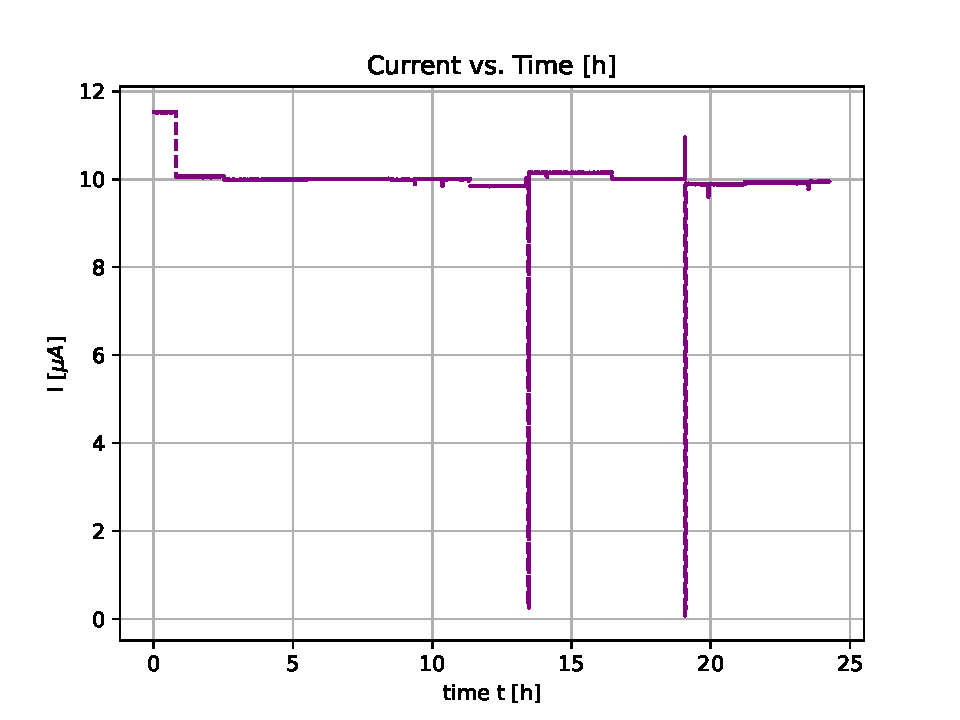
\includegraphics[width = 0.45 \textwidth]{Analysis/Dataselection/CurrentTrend.pdf}}
\subfloat[][\emph{$X,Y$ beam position over time} ]{
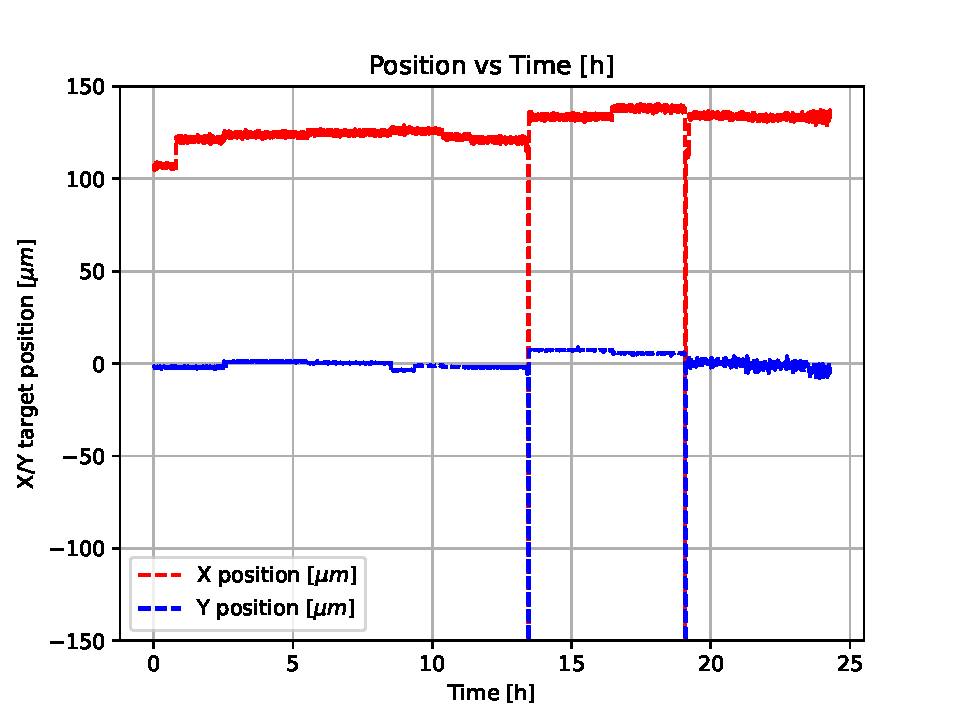
\includegraphics[width = 0.45\textwidth]{Analysis/Dataselection/XYtrend.pdf}}
\caption{On the left, current trend versus time for all the runs acquired. On the right the X and Y position versus time.}\label{fig::PositionTrend}
\end{figure}

Now we focus our attention on the correlated-difference values. These quantities, are used as independent variables for the fit, as explained before, are defined as 

\begin{align*}
\delta x =  \frac{(X_{up,1} + X_{up,2})}{2} - \frac{(X_{down,1} + X_{down,2})}{2}
\end{align*}

and are calculated within each single event, to identify the differences with respect to the various quantities such as position, energy, etc., which correspond to different states of polarization. For each of these quantities a correspondent histogram is shown in figure \ref{fig:BeamParameters}. These plots are useful to quantify the stability of the beam: we expect that all the correlated differences are distributed around zero, which implies that there is no systematic difference when the beam has one polarization state with respect to the other. The mean $\mu$ and the standard deviation $\sigma$ of the distributions are reported in the table (\ref{Tab:parametri}) 

\begin{figure}[!hbtp]
\centering 
\subfloat[][\emph{$X$ position correlated difference}]{
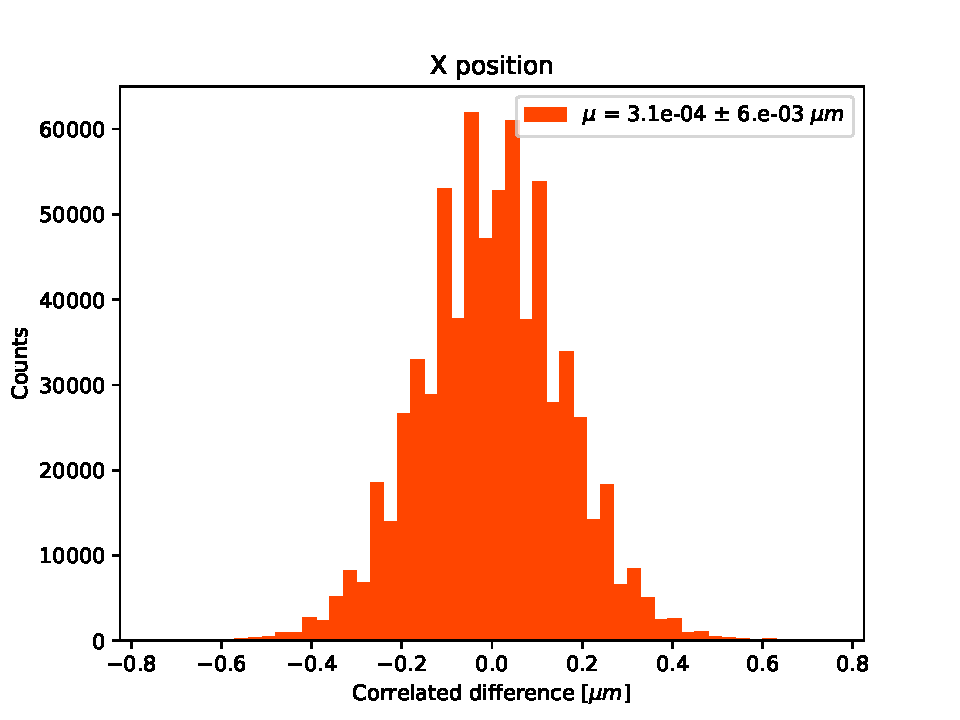
\includegraphics[width = 0.5\textwidth]{Analysis/Dataselection/X.pdf}} 
\subfloat[][\emph{$Y$ position correlated difference}]{
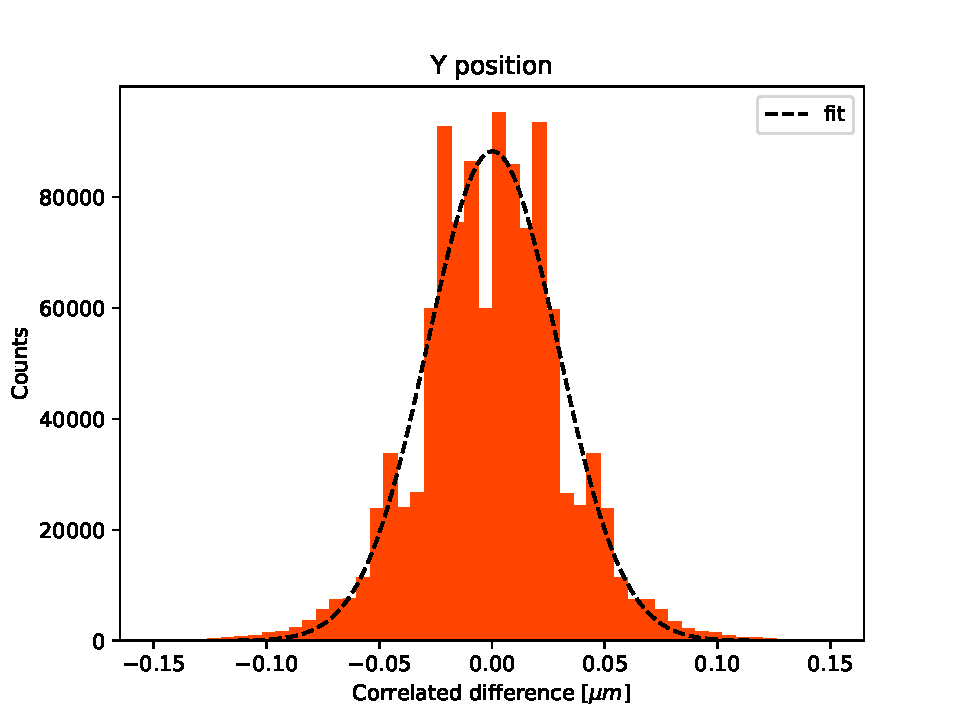
\includegraphics[width = 0.5\textwidth]{Analysis/Dataselection/Y.pdf}}\\
\subfloat[][\emph{$\theta_{x}$ correlated difference}]{
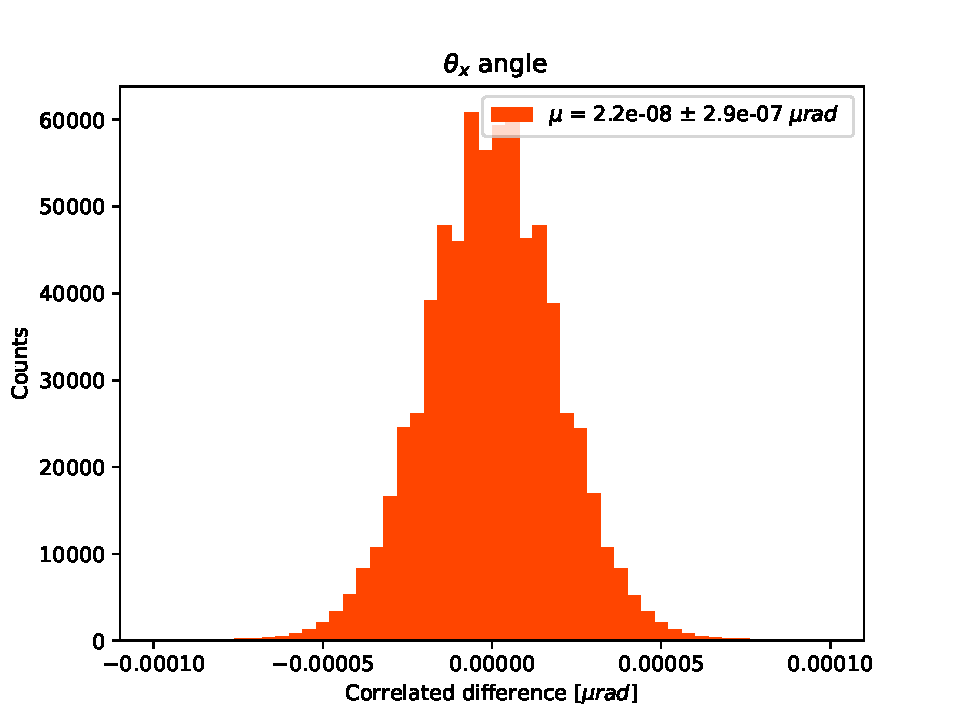
\includegraphics[width = 0.5\textwidth]{Analysis/Dataselection/Xp.pdf}} 
\subfloat[][\emph{$\theta_{y}$ correlated difference}]{
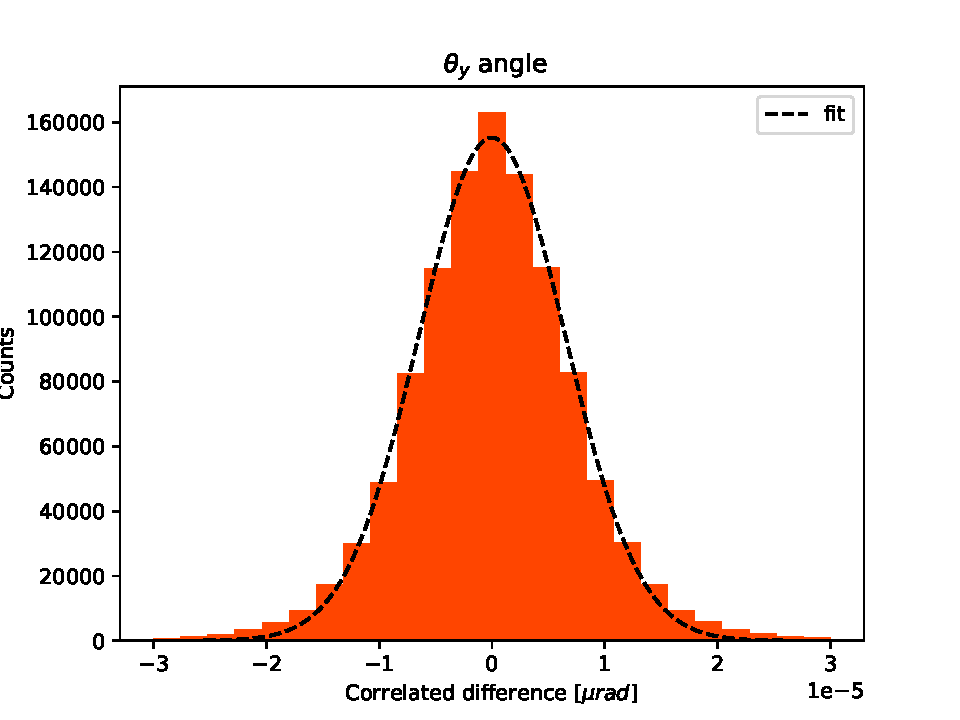
\includegraphics[width = 0.5\textwidth]{Analysis/Dataselection/Yp.pdf}}\\
\subfloat[][\emph{Energy correlated difference}]{
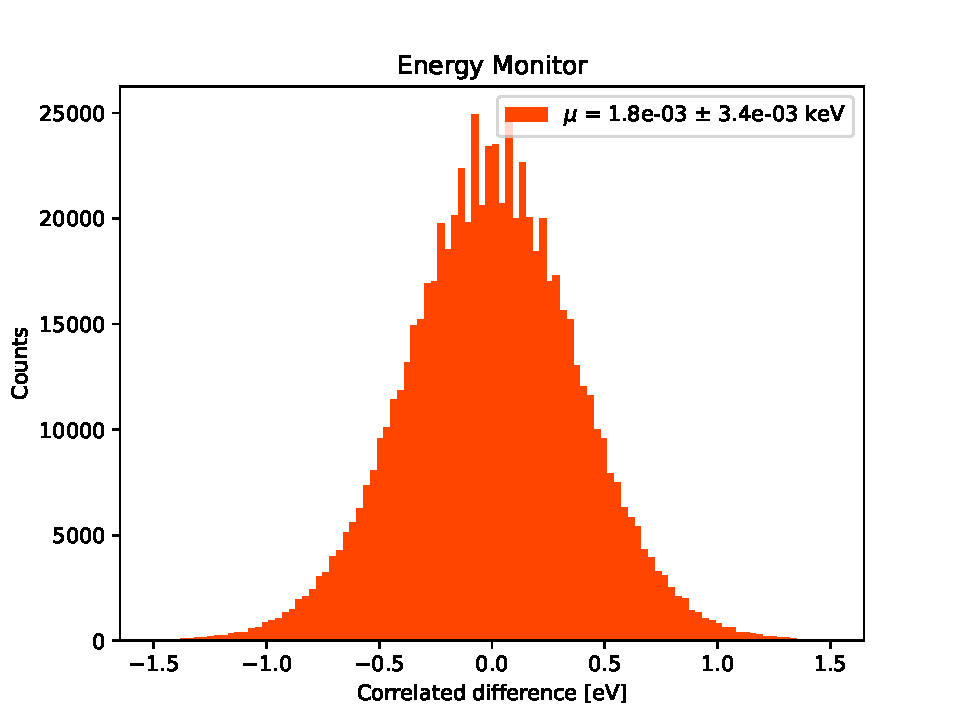
\includegraphics[width = 0.5\textwidth]{Analysis/Dataselection/ENMO.pdf}}
\subfloat[][\emph{Current asymmetry}]{
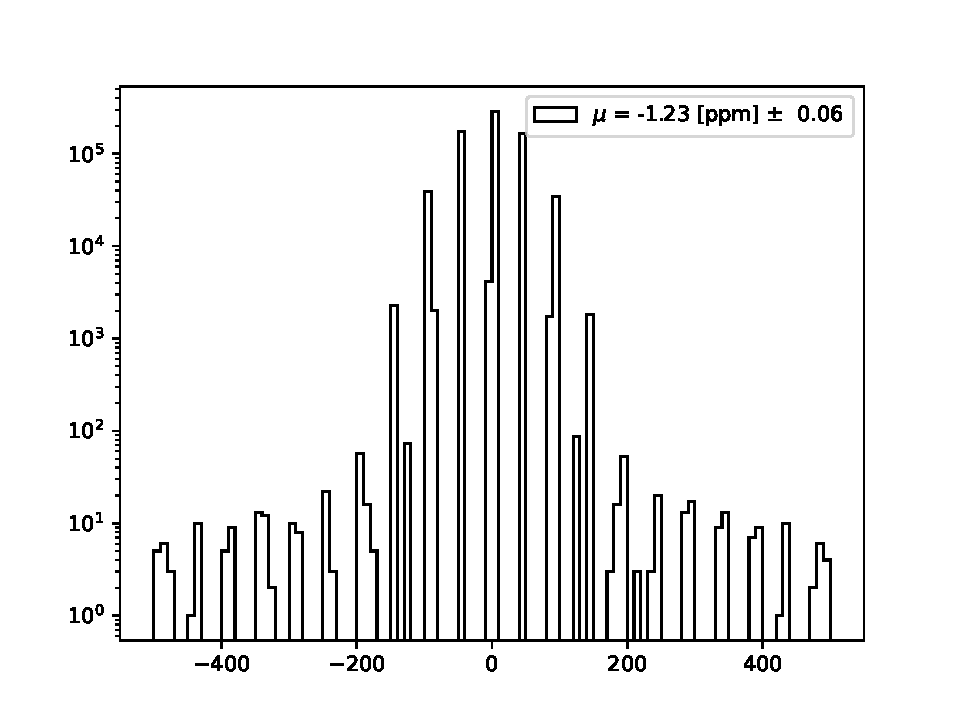
\includegraphics[width = 0.5\textwidth]{Analysis/Dataselection/Current.pdf}}
\caption{Histogram for the beam parameters.}
\label{fig:BeamParameters}
\end{figure}

Every histogram is generated with $100$ bins. For the current asymmetry, we discovered that the values of the VFCs resistance, which controls $V_{ref}$ value, was set too high. The resolution of this monitor is low, compared to the others, as we can see in the corresponding histograms, where the data are distributed around isolated peaks. This suggest to increase $V_{ref}$ of the VFCs, for the incoming experiment, to achieve a precision comparable with the other monitors.

\begin{table}[hbtp]
\centering
\caption{Beam parameters:}
\begin{tabular}{c|c|c|c|c|c|c} 
\hline 
\rule[-1ex]{0pt}{2.5ex} 
Beam Parameters &  $X [\mu m]$ & $Y[\mu m]$ & $ \theta_{x} [\mu rad]$ & $ \theta_{y} [\mu rad]$ & $E [eV]$ & $I [ppm] $ \\ 
\hline 
\rule[-1ex]{0pt}{2.5ex} $\mu$ & $1.31 \cdot 10^{-3}$ & $2.4 \cdot 10^{-4}$ & $3.2 \cdot 10^{-8} $ & $3.6 \cdot 10^{-9}$ & $0.0013$ & $-1.23$ \\ 
\hline 
\rule[-1ex]{0pt}{2.5ex} $sigma$ & $3.7 \cdot 10^{-1}$ & $2.9 \cdot 10^{-2}$ & $ 1.9 \cdot 10^{-5} $ & $6.5 \cdot 10^{-6}$ & $0.38$  & $50.4$ \\ 
\hline 
\end{tabular}
\label{Tab:parametri} 
\end{table}

Looking at the values of the mean and the corresponding error $\sigma$ reported in the plots legend, we observe that the means of $X,Y,\theta_{x},\theta_{y},E$ are compatible with $0$. These results are encouraging: we are not able to identify a systematic difference between polarization $+1$ and $-1$. A systematic difference would have produced a value $\mu$ shifted from zero, and a corresponding effect on $A_{n}$. 
With our assumption that the false asymmetries are well described by a linear model, observing that $\mu$ is small and compatible with zero for all the parameters, together with the evidence that $\delta q$ are distributed symmetrical around zero, leads to the cancellation of all the false asymmetries, as can be seen in equation \ref{eq:CancelOut} :

\begin{align} \label{eq:CancelOut}
\overline{A} = A_{n} \cdot P + \overline{\delta_{I}} + \overline{\delta_{x}}A_{x} + & \overline{\delta_{y}} A_{y} + \overline{\delta_{\theta_{x}}} A_{\theta_{x}} + \overline{\delta_{\theta_{y}}} A_{\theta_{y}} + \overline{\delta_{E}}A_{E} = A_{n} \cdot P + \overline{\delta_{I}}
\end{align}  

We will discuss later, when we will introduce the fit results, whether our assumption reflects the reality. We assume that the only false asymmetry that has an effect is $\delta I$: $\overline{\delta I}$ is equal $-1.23 \, ppm$, and we will subtract that to the final result:

\begin{align*}
A_{n} = \overline{A_{tot}} - \overline{\delta I}
\end{align*}

\newpage
\newpage
\section{Polarization Loss}

After discussing the removal of the outliers, now will discuss in details the issue regarding the polarization of the beam. To observe a transverse asymmetry, it is essential to have a correctly polarized beam. Unfortunately, we found out that  part of the data were acquired by mistake with a non-polarized beam. The reason is that during the second night of the experiment, MAMI operators who controls the quality of the beam, switched from polarized beam to non-polarized, unintentionally. These wrong data were acquired during the night of 2nd December and we discovered this problem only the next day. We had no indication of how many hours of beam were lost. Since this happened during the night, nobody could save the polarization measurement, and identify the runs affected by this problem.
This issue introduces a big systematic error that decreases the measurement of $A_{n}$. To proceed in the analysis, it is important to identify the runs sharing this problem, otherwise the measurements are affected by a bias that is not possible to disentangle from other systematic effects related to the electronics system of the experiment. 
All the stabilization monitors were active and the data apparently show the same behaviour of the data with the correct polarization. We can not proceed with an arbitrary cut of the data, because there is the risk to cut off also good data or perform an incomplete removal. The next phase of the analysis is focused on describing a method used to identify the data taken with unpolarized beam and remove them from the analysis.
 
The procedure to identify the runs without polarization rely on the estimation of the correlation coefficient of the PMTs counts. For every event we have two type of polarization sequence. The polarization $P$ of each sub-event is identified with $+1$ and $-1$, that correspond to up and down $P$. This values are part of the data tree, and form a sequence $p_{i}$ of the type: $+1-1-1+1$, where i is the index to the i-th sub-events analyzed. If the actual $P$ is different from zero, we expect a difference in the number of scattered electrons between sub-events with different $p_{i}$, caused by the transverse asymmetry (see table \ref{tab:PolarizationSequence}).

\begin{table}[hbtp]
\centering
\begin{tabular}{c|c|c|c|c|c|c|c|c}
\hline 
sub-event & 1 & 2 & 3 & 4 & 5 & 6 & 7 & 8 \\ 
\hline 
Polarity & +1 & -1 & -1 & +1 & +1 & -1 & -1 & +1 \\ 
PMT B0 & 101 & 99 & 98 & 102 & 100 & 99 & 97 & 103 \\ 
Other PMT & ... & ... & ... & ... & ... & ... & ... & ... \\ 
\hline
\end{tabular}
\caption{Example of the Polarity sequence and PMT counts that are saved in the analysis program. The values of the PMT counts given are for example.}
\label{tab:PolarizationSequence}
\end{table}

This leads to a positive/negative correlation between the sequence $p_{i}$ and the PMT data. In case of $P = 0$, the expected values for the correlation should be zero.
We applied this strategy with the hope to identify the blocks of data with $P = 0$, also using the knowledge that the polarization was turned off at some point during the night. The correlation $c$ between $p_{i}$ and the PMT sequence $N_{i}$ of counts is measured every $t = 1 h$, corresponding to $45000$ events. We plot the averaged correlation for detector A and B, and the correlation of the two detectors together (with the reverse sign for detector B) in figure \ref{fig:PolarityCheck}.

\begin{figure}[!ht]
\centering
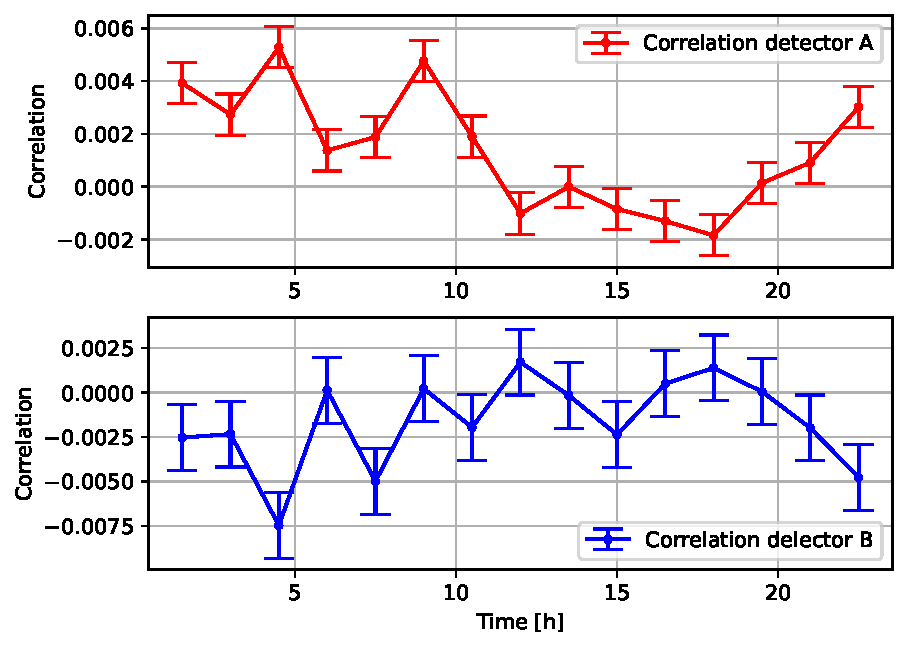
\includegraphics[width = 0.9\textwidth]{Analysis/Dataselection/Correlation.pdf}
\caption{Correlation between the polarization sequence and the asymmetry data. The correlation are measured for each data run, \SI{1}{\hour} long.}
\label{fig:PolarityCheck}
\end{figure}

\begin{figure}[!ht]
\centering
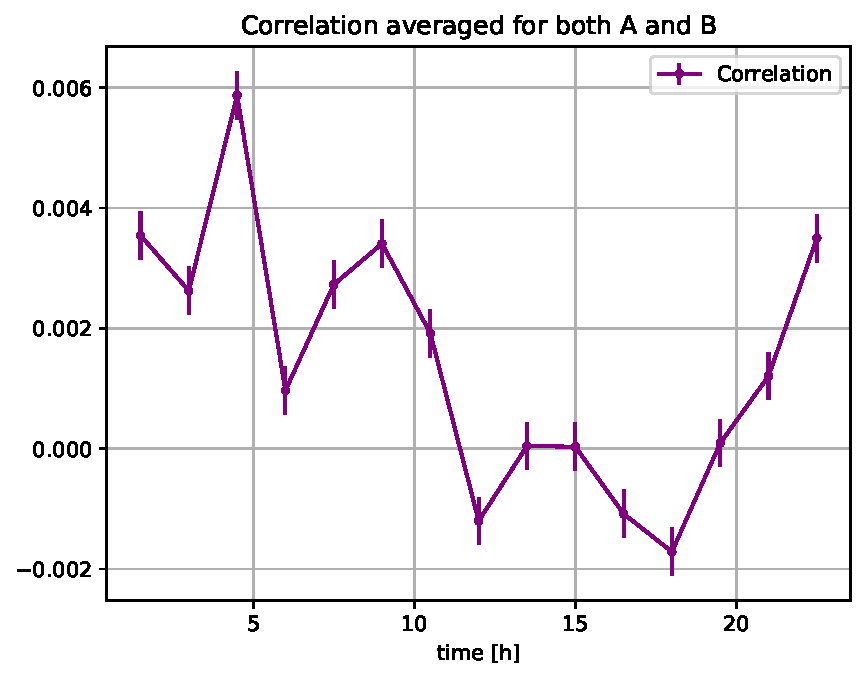
\includegraphics[width = 0.5\textwidth]{Analysis/Dataselection/OverallCorr.pdf}
\caption{Correlation between the polarization sequence and the asymmetry data. The plot shows the overall result for the two detector combined, reversing the sign of the asymmetries of detector B, together with the values expected from a Monte Carlo simulation. In yellow the error band computed with the Monte Carlo.}
\label{fig:PolarityCheck2}
\end{figure}

If we observe that $c$ is compatible with zero, we have an indication of the block of runs to be removed from the analysis.
The values are reported in figure \ref{fig:PolarityCheck}. The errors for each point are computed with the formula:

\begin{align*}
\sigma_{c} = \sqrt{\dfrac{1 - c^{2}}{N - 2}}
\end{align*} 

The plots show the expected values for the correlation coefficient, computed with a simple simulation, using the values of $A_{n} = 22.5 ppm$ and $P = 0.79$ as an input. The simulation results are obtained following these steps:

\begin{itemize}
\item A sequence of the type $+1,-1,-1,+1$ is generated, long $45000$ events.
\item For each sub-event of the previous sequence, the PMT counts are generated: the counts are sampled from a gaussian distribution with $\mu$ and $\sigma^{2}$ equal to the values measured for both the detectors. To reproduce the correlation with the polarity sequence, the values are shifted accordingly  by a factor $\mu \cdot A_{n} \cdot P$  
\item The previous step is repeated 25 times, and for each iteration we compute and save the correlation between the polarity sequences and the counts.
\item From the values saved, we compute the mean $c$ (the dotted line in plot \ref{fig:PolarityCheck}) and $\sigma_{c}$.
\end{itemize}

Looking at the plots, we observe for detector A a block of runs where $c$ is compatible with 0, in contrast with the values expected from the simulation. Due to the higher error, the corresponding plot for detector B is not clear to interpret, however the plot on the right with the overall results for A and B confirms the evidence for A.
This let us to identify the block of runs that show a behaviour compatible with $P = 0$. it is important to check that validity of this method seeing if the corresponding asymmetry is compatible with $0$ (see figure \ref{fig:ZeroAsym}).

\begin{figure}[hbtp]
\centering
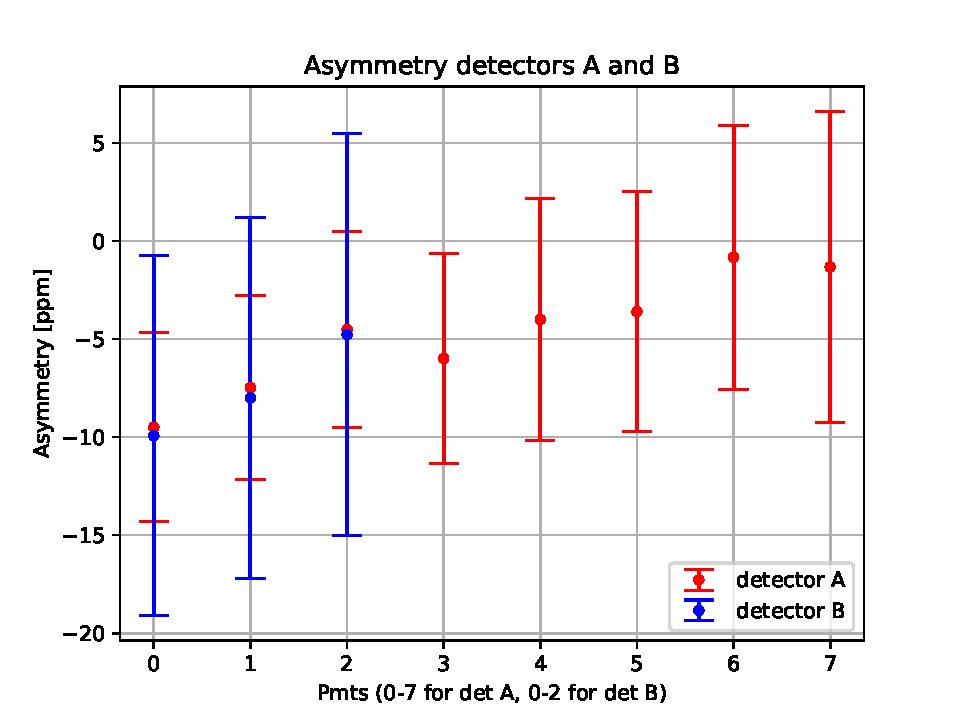
\includegraphics[width= 0.5\textwidth]{Analysis/Dataselection/Nopolarity.pdf}
\caption{Raw-asymmetry computed for the block of runs with $P = 0$. Except for one PMT of detector A, all the values are compatible with $0$ in $1\sigma$.}
\label{fig:ZeroAsym}
\end{figure}

The asymmetry values for this block of runs show an unexpected behaviour. For both detectors we observe negative values. The weighted mean for the two detector is :
\begin{itemize}
\item $A_{B} = -7 \pm 5$ ppm
\item $A_{A} = -5 \pm 2$ ppm
\end{itemize}

The values are not compatible with zero, but are compatible with each other. It is therefore reasonably certain that such data should not be included in the main analysis, because we observe a negative asymmetry for both the detectors that is not compatible with the presence of a polarized beam.

\section{Fit with a Linear Model}

At this point, it is interesting to study the distribution of the asymmetries measured by the two detectors. Our main assumption is that the asymmetries values are distributed following a normal distribution, around the physical value $A_{n}$. We have produced several histograms for the measurements of every PMT (see figure \ref{fig:AsymmtriesB0B1B2},\ref{fig:AsymmtriesA0A1A2A3} and \ref{fig:AsymmtriesA4A5A6A7}). The data without polarization are not included in the histograms. For every histogram we use a gaussian function to fit the data, the reduced $\chi^{2}$ is reported in table \ref{tab:Chisq}.
We see a good agreement with the hypothesis of normally distributed data.

\begin{figure}[!ht]
\centering
\subfloat[][]{
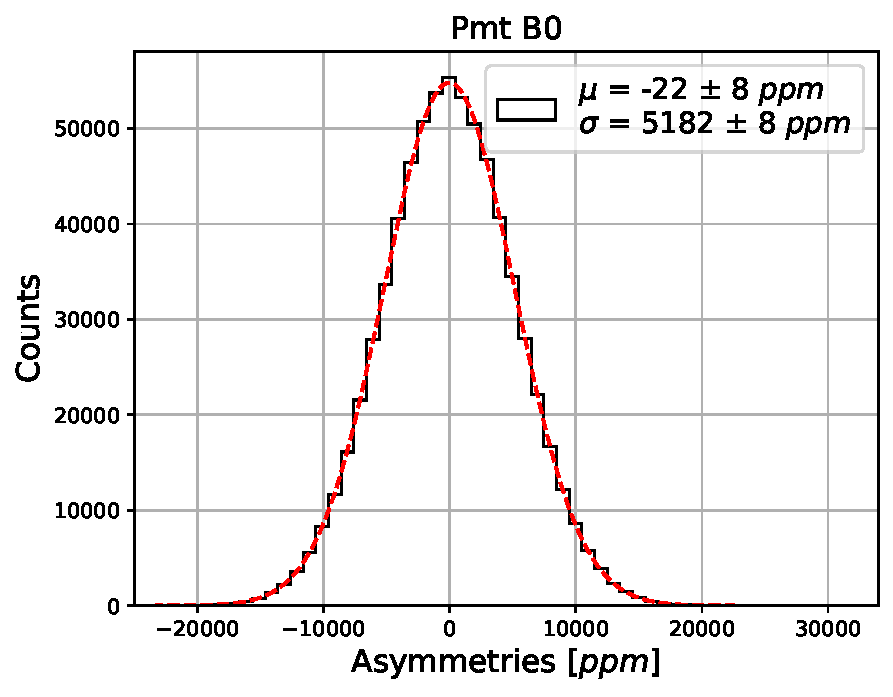
\includegraphics[width = 0.4\textwidth]{Analysis/Histogram/B0.pdf}}
\subfloat[][]{
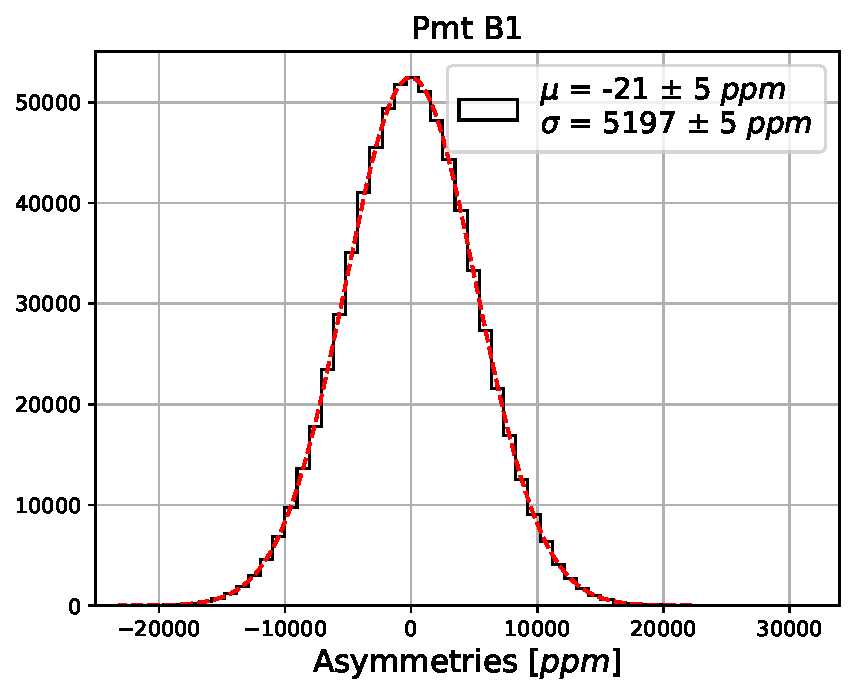
\includegraphics[width = 0.4\textwidth]{Analysis/Histogram/B1.pdf}}\\
\subfloat[][]{
\includegraphics[width = 0.4\textwidth]{Analysis/Histogram/B2.pdf}
}
\caption{Histogram of the Asymmetry for Detector B. The Asymmetries are corrected removing the data without polarization. The raw asymmetries are multiplied by $\frac{1}{P}$}
\label{fig:AsymmtriesB0B1B2}
\end{figure}

\begin{figure}[!ht]
\centering
\includegraphics[width = 0.40\textwidth]{Analysis/Histogram/A0.pdf} 
\includegraphics[width = 0.40\textwidth]{Analysis/Histogram/A1.pdf}\\
\includegraphics[width = 0.40\textwidth]{Analysis/Histogram/A2.pdf} 
\includegraphics[width = 0.40\textwidth]{Analysis/Histogram/A3.pdf}
\caption{Histogram of the Asymmetry A0,A1,A2,A3.The Asymmetries are corrected removing the data without polarization. The raw asymmetries are multiplied by $\frac{1}{P}$}
\label{fig:AsymmtriesA0A1A2A3}
\end{figure}

\begin{figure}[!ht]
\centering
\includegraphics[width = 0.40\textwidth]{Analysis/Histogram/A4.pdf}
\includegraphics[width = 0.40\textwidth]{Analysis/Histogram/A5.pdf}\\
\includegraphics[width = 0.40\textwidth]{Analysis/Histogram/A6.pdf}
\includegraphics[width = 0.40\textwidth]{Analysis/Histogram/A7.pdf}
\caption{Histogram of the Asymmetry for Detector A.}
\label{fig:AsymmtriesA4A5A6A7}
\end{figure}

\begin{table}[!h]
\centering
\begin{tabular}{c|c}
\hline 
Pmt & reduced $\chi^{2}$ \\ 
\hline
B0 & $1.2 \pm 0.2$ \\ 
B1 & $0.9 \pm 0.2$ \\ 
B2 & $1.2 \pm 0.2$ \\
A0 & $1.2 \pm 0.2$ \\ 
A1 & $0.7 \pm 0.2$ \\ 
A2 & $0.7 \pm 0.2$ \\ 
A3 & $0.9 \pm 0.2$ \\ 
A4 & $1.4 \pm 0.2$ \\ 
A5 & $0.7 \pm 0.2$ \\ 
A6 & $1.1 \pm 0.2$ \\ 
A7 & $1.7 \pm 0.2$ \\ 
\hline 
\end{tabular}
\caption{Reduced $\chi^{2}$ for the gaussian fit of the asymmetry data.} 
\label{tab:Chisq}
\end{table}

Recalling equation \ref{eq:Error}, where we assumed that $A$ is a normally distributed variable, now we can confirm our initial assumption. To extract the asymmetry $A_{n}$ from the data, we assume a linear model where the asymmetries depend on the beam parameters, in the way we discussed in section \ref{Model}. The contributions due to variations of the beam within an events are described with 5 parameters, that are  $A_{x},A_{y},A_{\theta_{x}},A_{\theta_{y}},A_{E}$.
The data are analyzed both using python libraries, and with a fit program implemented in the framework of this thesis. To analyze the data with python, it is used the \textit{curvefit} function implemented in the python library \textit{scipy}. We also implemented a dedicated program to interface directly to the analysis program, the fit program, that is written in \textit{C++} code. The fit program implements the ordinary least square algorithm (OLS), a well know algorithm used in linear regression. The OLS algorithm is a basic algorithm, easy to implement and robust. In linear regression it is assumed that :

\begin{equation}
 y \, = \, \vec{x} \cdot \vec{\beta} + \epsilon
\end{equation}

$\vec{x}$ are the independent variables, $\vec{\beta}$ are the parameters and $\epsilon$ is a noise parameter, that is supposed to be gaussian (however, the robustness of the OLS algorithm allows relaxing this request). Another important assumption is that the linear variables are not correlated. 
This last requirement is particularly important, as correlated data can not be processed with either of the two algorithms used. Before proceeding with the fit, it is necessary to verify this assumption. The correlation matrix for the beam parameters is reported in a table \ref{tab:CorrMatrix}.

\begin{table}[!h]
\centering
\begin{tabular}{c|cccccc}
\hline 
             & $X$ & $Y$ & $\theta_{x}$ & $\theta_{y}$ & $E$ & $I$\\ 
\hline 
$X$            & 1 & -0.02 & -0.99 & 0.06 & 0.04  & -0.03\\ 

$Y$            & -0.02 & 1 & 0.01 & -0.65 & 0.01  & -0.02\\ 

$\theta_{x}$ & -0.99 & 0.006 & 1  & -0.005 & -0.05 & 0.03\\ 

$\theta_{y}$ & 0.06 & -0.65 & -0.05 & 1 & -0.003  & 0.03\\ 
 
$E$            & 0.04 & 0.005 & -0.05  & -0.003  & 1 & 0.26\\ 
 
$I$            & -0.03 & -0.02 & 0.03  & 0.03 & 0.26 & 1\\ 
\hline
\end{tabular}
\caption{Correlation coefficient between beam parameters.}
\label{tab:CorrMatrix} 
\end{table}

The correlation between $(\theta_{x},X);(\theta_{y},Y)$ the values for the correlation are high compared to the other parameters. 

\begin{figure}[!ht]
\centering
\subfloat[][\emph{}]{
\includegraphics[width = 0.5 \textwidth]{Analysis/Fit/X_Xp.pdf} }
\subfloat[][\emph{}]{
\includegraphics[width = 0.5 \textwidth]{Analysis/Fit/Y_Yp.pdf}} \\
\subfloat[][\emph{}]{
\includegraphics[width = 0.45 \textwidth]{Analysis/Fit/Y_X.pdf}}
\caption{Correlation plots of positions and angles.}
\label{fig:CorrelationBeam}
\end{figure}

The plots in figure \ref{fig:CorrelationBeam} confirm the linear dependence between the parameters. For the $\theta_{x}$ versus the $X$ position the data are distributed on a line, with complete anti-correlation. For the $\theta_{y}$ versus $Y$, the data are distributed following parallel lines, that have the same angular coefficient but different offsets. The lines are equally spaced, meaning that the beam parameter $\delta Y$ is translated, for a fraction of the events, by a multiple of some quantity $\delta l_{y}$. With the linear fit we estimate that $\delta l_{y} = 0.017 \pm 0.001 \, \SI{}{\micro \meter}$. This effect could reproduce the data structure that we observe in plot \textit{b} of figure \ref{fig:CorrelationBeam}. 

\commento{
\begin{figure}[hbtp]
\centering
\includegraphics[width = 0.5 \textwidth]{Dataselection/XXp_time.pdf}
\caption{Plot of the $\delta X$ and $\delta \theta_{x}$ normalized versus event. The beam parameters in figure are anti-correlated.}
\label{fig:XXpvsTime }
\end{figure}}

It is clear that we have to modify the model to fit the data. We decided to include as linear independent variables only : $I,X,Y,E$. Before proceeding with the fit, it is interesting to study how $A_{n}$ evolves increasing the data size. This can be seen by plotting the averaged values $\overline{A_{n}}$ as the number of events increases, where the average is made on all data collected from time $t = 0$ up to time $t = t_{1}$, as shown in figure \ref{fig:AsymOverTime}. 

\begin{figure}[!hbtp]
\centering
\subfloat[][\emph{Averaged asymmetries for each PMT.}]{
\includegraphics[width = 0.5 \textwidth]{Analysis/Dataselection/AveragedAsymmetry.pdf}}
\subfloat[][\emph{Averaged asymmetry for detector A and B. The dotted line correspond to $1\sigma$ error.}]
{\includegraphics[width = 0.5 \textwidth]{Analysis/Dataselection/AveragedAsymmetry2.pdf}}
\caption{Plot of the Asymmetry versus time. The plot show the average over all the events collected from $t = 0$ to $t = t_{1}$. Each line represents $A_{n}$ measured for  PMT (in \textcolor{blue}{blue} detector B and in \textcolor{red}{red} detector A). The values are corrected for the beam polarization, multiplying by $\frac{1}{p}$. No further correction is applied.}
\label{fig:AsymOverTime}
\end{figure}

These plots are useful to check that the asymmetries converge to a certain value, and that there are no steep variations that could be related to the presence of remaining outliers. We observe that the sign of the asymmetries for the two detectors are opposite, in agreement with what we expect from the different kinematics, with the sign of the asymmetry given by the sign of the projection of the cross product $\vec{k} \times \vec{k}'$ along the axis orthogonal to the scattering plane. For detector A the cross product projection is positive, while for the detector B it is negative.
For a better visualization of the data, especially to observe the dependence of the asymmetry on the beam parameters measured, it is useful to plot $A$ versus each of the beam parameters. Unfortunately, the statistical error associated to the asymmetry is too high to appreciate whether there is a linear dependence in the data. For example, in figure \ref{fig:AsymmetryA0vrX} we plot the asymmetries $A$ versus $X$.

\begin{figure}[!hbtp]
\centering
\includegraphics[width = 0.75\textwidth]{Analysis/Fit/A_vs_X.pdf}
\caption{Detector A asymmetries versus X beam position. Because of the statistical uncertainties, it is not possible to visualize a linear dependence in the data. Each dot is colored depending on the density of points.}
\label{fig:AsymmetryA0vrX}
\end{figure}

The statistical error associated to $A$ is too high to identify a trend in the values. A different approach is to divide the $x$ axis in small intervals, and average the asymmetries in each interval. In a plot of this type each point represents the overall asymmetry for a particular interval of $X$ ,$Y$ or $E$.
 
\begin{figure}[!hbtp]
\centering
\subfloat[][]{ 	\includegraphics[width = 0.45\textwidth]{Analysis/Fit/pmtA0_X.pdf}}
\subfloat[][]{ 	\includegraphics[width = 0.45\textwidth]{Analysis/Fit/pmtA0_Y.pdf}}\\
\subfloat[][]{ 	\includegraphics[width = 0.45\textwidth]{Analysis/Fit/pmtA0_E.pdf}}
\caption{ $A$ versus $\delta x$, $\delta y$ and $\delta E$. The plot are generated with 50 equally spaced bins. The red line is the best fit with a linear model.}
\end{figure} 

We report for brevity only the values for PMT A0 of detector A. In this case is simpler to identify the presence of a linear dependence in the data. The errors are computed with the formula defined in equation \ref{eq:Error}, considering each interval separately.
Another approach that we used to further reduce the fluctuations related to the statistical error of $A_{n}$ is an additional average over all the PMTs of each detector. The result is shown in figure \ref{fig:DifferentModels}.

\begin{figure}[!ht]
\centering
\subfloat[][\emph{ $A$ versus $\delta x$}]{ \includegraphics[width = 0.5\textwidth]{Analysis/Fit/Xfit.pdf}}
\subfloat[][\emph{ $A$ versus $\delta y$}]{ \includegraphics[width = 0.5\textwidth]{Analysis/Fit/Yfit.pdf}}\\
\subfloat[][\emph{ $A$ versus $\delta E$}]{ \includegraphics[width = 0.5\textwidth]{Analysis/Fit/Efit.pdf}}
\caption{Averaged asymmetries versus the beam parameters $\delta X$, $\delta Y$ and $\delta E$. The x axis is divided in $19$ intervals, and for each of them we average the asymmetries $A$. The linear model is the red line, the second used to fit the data is a polynomial, represented in blue. }
\label{fig:DifferentModels}
\end{figure}

 This procedure decreases the error of a factor $\sqrt{8}$ for detector A and $\sqrt{3}$ for detector B. However, this does not take into account the different linear dependencies on the beam parameters for the various PMTs, and therefore is not immune from a possible bias. 
We have explored different models to describe the asymmetry dependence on beam parameters. The first one is the linear model: 

\begin{equation}
A = A_{x} \, \delta x + A_{phys}
\end{equation}

For $X$ and $Y$ positions, we tried to use a 5th order polynomial:

\begin{equation}
A = c \, \delta x^{5} + A_{x} \, \delta x + A_{phys}
\end{equation}

While for the energy monitor, we tried a 3rd order polynomial:
\begin{equation}
A = c \, \delta E^{3} + A_{E} \, \delta E + A_{phys}
\end{equation}

The choice of an odd exponent is due to the observation that $A$ increases near the edges of the plot with opposite sign.
The values of the fit parameters are reported in the plots of figures . The $\chi^{2}$ of the fit are reported in table \ref{tab:ChisqDiffModel}

\begin{table}[!ht]
\centering
\begin{tabular}{c|c|c|c}
\hline 
detector A & $X$ & $Y$ & $E$ \\
\hline 
linear fit $\chi^{2}_{17}$ & 99 & 59 & 94 \\ 
alternative model $\chi^{2}_{16}$ & 76 & 55 & 78 \\ 
\end{tabular}
\caption{$\chi^{2} _{ndf}$ for the different models used to fit the data show in figure \ref{fig:DifferentModels}}
\label{tab:ChisqDiffModel}
\end{table}

The $\chi^{2}$ values are higher that the expected and we observe that the values for the model 2 are lower than the ones of linear fit.
This high values can be explained with two considerations: the first one is that this procedure of averaging the data based on $x$ interval leads to the loss of information that can influence the fit, the second consideration is that we are ignoring the possible error in the determination of $\delta x$.
Despite of this, we observe that using a model with more complicated dependencies does not change  the values of $A_{phys}$. Therefore we do not see a strong reason to change the linear model. The model that is used to extract the asymmetry is given in equation \ref{eq:ModelloUsato}. 

\begin{equation} \label{eq:ModelloUsato}
A_{tot} = A_{phy} \cdot P + \delta_{I} + A_{x} \delta x + A_{y} \delta y + A_{E} \delta E 
\end{equation}

\commento{
\begin{equation} \label{eq:ComplicatedModel}
A_{tot} = A_{phy} \cdot P + \delta_{I} + A_{x} \delta x + A_{y} \delta y + A_{E} \delta E + c_{x} \, \delta x^{5} + c_{y} \, \delta y^{5} + c_{E} \, \delta E ^{3}
\end{equation}}

the result of the fit are reported in table \ref{tab:resultA}, together with the final result of the asymmetry for detector A and B.



\section{False Asymmetries}

In the data analysis, the values of the false asymmetries have been threated as parameters of the linear fit. In this section we will investigate how we can obtain another different estimations, useful to check the validity of all the process of analysis of the data.

For $\frac{dA}{dX}$ and $\frac{dA}{dY}$, we conceptually exploit the possibility of varying the position of the beam on the target, as we did during one of the calibration phases. Using the same \textit{wobbler 16} we asked MAMI to slowly change the beam position on the X and Y monitor. The change in position has the effect to modify the rates for the two detector, and from them it is possible to extract estimate the two false asymmetries related to the beam position. Now we will see how the two quantities are related.
From the plot \ref{fig:SlowPosition} we see that the counts are changing linearly with the beam position, so we assume that the $N$ are given by

\begin{align*}
N(x,...) = N_{0} + m \cdot (x - x_{0})
\end{align*}

it is clear that the linear model has limits, and at some point the electron will be deflected completely out of the detector, with the counts will falling rapidly to zero. However, the magnets used to deflect the beam are producing small variation in the position, on the order of hundredths of a millimeters.
Let's suppose that the beam position for two sub-events is $x_{1}$ and $x_{2}$, we can calculate the asymmetry between the two event, taking care of the possible effects due to the different position. We write explicitly: 

\begin{equation}
\begin{split}
Asym = \dfrac{N(x_{1}) - N(x_{2})}{N(x_{1}) + N(x_{2})} = \dfrac{N_{0} + m \cdot (x_{1} - x_{0}) - N_{0} - m \cdot (x_{2} - x_{0})}{N(x_{1}) + N(x_{2})} = \\ \dfrac{m}{2 N_{0} + m \cdot (x_{1} +  x_{2}) - 2m x_{0}}(x_{1} -  x_{2})
\end{split}
\end{equation}

In this equation three different parameters appear: $N_{0}$ is the offset of the linear model, $m$ is the angular coefficient, or the slope, and $x_{0}$ is the initial position respect to we compute the position variation. The first two terms are obtained by a linear fit, while $x_{0}$ is fixed conveniently.

\begin{figure}[hbtp]
\centering
\subfloat[][\emph{Plot for slow variation in $x$ direction for detector B.}]
{\includegraphics[scale=0.5]{Analysis/slowxVariation.pdf}}
\subfloat[][\emph{Plot for slow variation in $x$ direction for detector B.}]{\includegraphics[scale=0.5]{Analysis/slowyVariation.pdf}}
\caption{Plot of the PMT counts versus the $X$ position. The $X$ position was slowly changed during the acquisition.}
\label{fig:SlowPosition}
\end{figure}

If the values $x_{1}$ and $x_{2}$ are are distributed symmetrically \footnote{ In the same way of the beam parameter difference, shown in figure \ref{fig:BeamParameters}} We can simplify the denominator deleting the term $ m \cdot (x_{1} +  x_{2})$, fixing $x_{0} = \frac{x(1) + x(2)}{2}$. 

\begin{equation}
Asym = \dfrac{m}{2N_{0}}(x_{1} -  x_{2})
\end{equation}

The term in front of $(x_{1} - x_{2})$ can be compared to $\frac{dA}{dX}$. For $N_{0}$, the offset, we substitute the averaged value counts of each PMT for the polarized beam acquisitions.
The data are reported in the table \ref{tab:RateCarbon}:

\begin{table}[h]
\centering
\begin{tabular}{c|c|c}
\hline 
PMT & Detector A & Detector B \\ 
\hline
PMT 0 & 63733 & 17609 \\ 
PMT 1 & 67262 & 17514 \\ 
PMT 2 & 59782 & 14055 \\ 
PMT 3 & 51736 & \\ 
PMT 4 & 39057 & \\ 
PMT 5 & 39667 & \\ 
PMT 6 & 32768 & \\ 
PMT 7 & 23593 & \\ 
\hline 
\end{tabular}
\caption{Average counts per pmt, for time length of $\SI{20}{\milli \second}$.} 
\label{tab:RateCarbon}
\end{table}
 
The values for the false asymmetries obtained with this method are:

\begin{table}[h]
\centering
\begin{tabular}{c|c|c}
\hline
 'PMT' & $A_{x}$ $\SI{}{\per \micro \meter}$&   $A_{y}$ $\SI{}{\per \micro \meter}$ \\
\hline
 B0 & 692 & 795 \\
 B1 & 395 & 682 \\
 B2 & 289 & 601 \\
 A0 & 233 & 533 \\
 A1 & 223 & 518 \\
 A2 & 202 & 493 \\
 A3 & 190 & 473 \\
 A4 & 211 & 503 \\
 A5 & 214 & 506 \\
 A6 & 217 & 510 \\
 A7 & 220 & 514 \\
\hline
\end{tabular}
\caption{ Values for the false asymmetry, computed with the slow horizontal and vertical variation mode.}
\end{table}

These values are not in agreement with $A_{x}$ and $A_{y}$ obtained from the fit (\ref{tab:resultA}). This may be due to the high correlation with the $\theta_{x}$ beam parameter. The negative correlation with $\theta_{x}$ means that when $\delta X$ increases $\delta \theta_{x}$ decreases, and then the false asymmetries combined together. Using linear regression, it is not possible to disentangle the effects of the correlation in the data, and therefore the corresponding coefficient of the fit are not reliable. 

\subsection{Energy Asymmetry}

For the energy asymmetry, a different method is necessary. We directly compute the Mott cross-section of the electron-carbon elastic scattering, and from that we can derive the false asymmetry due to energy variation.
We start from the formula of the expected rates:

\begin{equation}
\frac{events}{time} = n_{e} N_{t} v_{e} \frac{\partial \sigma}{\partial \Omega} (\Delta \Omega_{a}) \epsilon 
\end{equation} 

Where:
\begin{itemize}
\item $n_{e}$ electron density of the beam.
\item $N_t$ Number of scattering centers of the carbon target.
\item $v_{e}$ electron speed.
\item $\Delta \Omega_{a}$ solid angle acceptance of the spectrometers.
\item $\epsilon$ detector efficiency.
\end{itemize}

We do not need to compute directly the expected rate for the two detectors, because some terms cancel out when substituted in the formula for the asymmetry, the only relevant term is the cross section:

\begin{align*}
A = A_{n} + \dfrac{\sigma(E_{1}) - \sigma(E_{2})}{\sigma(E_{1}) + \sigma(E_{2})}
\end{align*}

Because $\Delta \Omega_{a}$ is a common term in the numerator and in the denominator, we can simplify the expression and substitute $\sigma $ with $ \frac{\partial \sigma}{ \partial \Omega}$.
The Mott cross section is given by the formula below:

\begin{equation} \label{eq:Mott}
\dfrac{\partial \sigma}{\partial \Omega} = \dfrac{Z^{2} \alpha (\hbar c)^2}{E^{2} sin^{4}(\frac{\theta}{2})} \cdot \frac{E'}{E} \cdot  cos(\frac{\theta}{2}) \cdot F^{2}(\vec{q}) 
\end{equation}

Where the first term is the Rutherford cross-section, the second term represent the recoil of the nucleus, the third terms is the $cos(\frac{\theta}{2})$, and the last term is the nucleus form factor. The Recoil term can be written:

\begin{align*}
\dfrac{E'}{E} = \dfrac{1}{1 + \frac{E}{Mc^{2}} (1 - cos(\theta))}
\end{align*}

With this final substitution we can rewrite the Mott cross section as:
\begin{align*}
\dfrac{\partial \sigma}{\partial \Omega} = \dfrac{D}{AE^{2}} \cdot \dfrac{1}{1 + EC} \cdot B \cdot F^{2}(\vec{q})
\end{align*}

Where $D = Z^{2} \alpha ((\hbar c)^2)$, $A = sin^{4}(\frac{\theta}{2})$ and $B = cos(\frac{\theta}{2})$. To compute the false asymmetry related to energy, we always assume that for small energy variation, a first order approximation is valid:

\begin{align*}
\sigma (E_{1}) \simeq \sigma(E_{0}) + \frac{\partial \sigma}{\partial E} (E_{1} - E_{0})
\end{align*}

The approximations is done for small variations around the beam energy, which is $\SI{570}{\mega \electronvolt}$.
Now it is possible to compute the false asymmetry, the searched expression is:

\begin{equation}
A_{E} = \dfrac{\partial \sigma}{\partial E \partial \Omega} \cdot  (2 \dfrac{\partial \sigma}{\partial \Omega})^{-1}
\end{equation}

We compute the above formula withe the constant A,B,C,D defined in \ref{eq:Mott}.

\begin{equation}
A_{E} = - \frac{1}{2} \dfrac{2 + CE_{0}}{E_{0} + E_{0}^{2}C} 
\end{equation}

Applying the above formula, we end with $A_{E} = -1.75 \, \frac{ppm}{\SI{}{\kilo \electronvolt}}$. We can compare this result with the values obtained from the fit, that are reported in table \ref{tab:resultA}. There is at least an agreement on the sign, with an expected negative effect related to the beam variation. However, the false asymmetries from the fit are one order of magnitude higher than the values computed here. An explanation could be that the energy variation is correlated to other beam parameters, or effects that are not considered in this analysis. Usually correlated data alters the result of the regression algorithms, which are not able to estimate the value of the coefficients. Looking at the values reported in table \ref{tab:CorrMatrix}, we observe a positive correlation between current and energy. Even if the correlation is not high, it still might cause a combination of effects which can be responsible for the lower values of $A_{e}$ measured with the fit.
Since it is not possible to compute analytically the correlation between the beam parameters parameters, the linear fit seems to be an easier method. An alternative approach may include Monte Carlo simulations of the beam, to take care of possible correlation between the various beam parameters, which in contrast are computationally expensive, compared to linear regression.

\section{Rates on Lead}

After all the calibrations are done, we proceeded with the measurement of the rates on lead target, one of the objectives of the experiment.
The lead target installed is made of a thin layer with a thickness of $\SI{0.5}{\milli \meter}$, and it is not isotopically pure.
We took $14$ acquisitions lasting $\simeq 2,5$ minutes, which corresponds to $6950$ events. For each of these acquisitions we set the beam current at different values, ranging from $\SI{10}{\micro \ampere}$ to $\SI{22}{\micro \ampere}$ of intensity. The rates are then reported as a function of the current and linear model is used to fit the data.

\begin{figure}[hbtp]
\centering
\includegraphics[width = 0.9\textwidth]{Analysis/LeadRates/LeadRates.pdf}
\caption{rates on lead Target as function of the beam current. The rates for each PMT of detector A (on the left), and detector B (on the right) are reported.}
\end{figure}

We fit using a linear model the data. The angular coefficient $m$ and the offset $q$ are reported in the table \ref{tab:LeadRates} for each PMTs of the two detectors.  

\begin{table}[ht]
\centering
\begin{tabular}{cccc}
\hline
 PMT   & m [$\SI{}{ \per \micro \ampere}$]          & q                &  $\chi^{2}$ (dof = 9) \\
\hline
 A0    & 501.4 +/- 2.2 & 257 +/- 40 & 13.8  \\
 A1    & 605.8 +/- 2.3 & 226 +/- 42 & 13.4  \\
 A2    & 495.0 +/- 1.5 & 163 +/- 27 &  7.0  \\
 A3    & 345.7 +/- 1.6  & 113 +/- 30  & 12.0 \\
 A4    & 232.6 +/- 0.9  & 74 +/- 16  &  5.4 \\
 A5    & 242.0 +/- 0.7 & 66 +/- 14  &  3.5  \\
 A6    & 205.8 +/- 0.7 & 52 +/- 12  &  3.1  \\
 A7    & 143.4 +/- 0.5 & 36 +/- 9   &  2.3  \\
 B0    & 92.6 +/- 0.3  & -17 +/- 6  &  2.1  \\
 B1    & 92.3 +/- 0.3  & -17 +/- 6   &  1.9  \\
 B2    & 68.5 +/- 0.3  & -9 +/- 6   &  2.8  \\
\hline
\end{tabular}
\caption{Lead rates, the values are measured for a target width of $\SI{0.5}{\milli \meter}$.}
\label{tab:LeadRates}
\end{table}

The PMT Counts with this target, increase from $100$ counts for detector B to $500$ counts every $\SI{1}{\micro \ampere}$. It is interesting to recover the formula of the experimental standard deviation $\sigma$ associated to the asymmetry distribution:

\begin{equation}
\sigma = \sqrt{\dfrac{1}{2 N \cdot n}}
\end{equation}

Where $N$ is the counts per sub-event, while  $n$ is the number of event analyzed.
Let's suppose that we want to obtain, for each PMTs, a statistical error not greater than $4,8 \, ppm$. With this accuracy, the overall result A will have an error given by $\frac{4.8 \, ppm}{\sqrt{8}} \simeq 1.7 \, ppm$, equal to the statistical error that we have obtained for the measurement of $A_{n}$ with $^{12}C$ ( see table \ref{tab:RisultatiBellissimiFinali}) while for detector B an overall result of $2.8 \, ppm$.
We have computed the time needed to achieve this accuracy for both detectors, given in total hours of experiment. This values are arbitrary: as shown in chapter \ref{result}, the transverse asymmetry on carbon has been measured with the same accuracy.  

\begin{table}[h]
\centering
\begin{tabular}{c|c|c}
\hline
   current I \SI{}{\micro \ampere} &   T [h] Det A &   T [h] Det B \\
\hline
        10   &       344 &      1487  \\
        12.5 &       277 &      1185   \\
        15   &       232 &      985 \\
        17.5 &       199 &      843 \\
        20   &       175 &      737 \\
\hline
\end{tabular}
\caption{Estimated time needed for the upcoming experiments to measure the transverse asymmetry for Lead with an aimed precision of $1.7 \, ppm$ for detector A and $2.8 \, ppm$ for detector B.}
\end{table}

The amount of time needed to obtain this accuracy with carbon is roughly $15 h$ with $\SI{10}{\micro \ampere}$. The same measurement with lead will need 23 times the time accumulated for Carbon. This is due to the fact that the target thickness for lead target must be smaller than the target thickness for carbon. Because the atomic number of lead is greater than carbon, the amount of radiation during the experiment is exponentially higher. During the experiment, the A1 experimental hall is constantly monitored, the radiation level can not exceed a certain threshold. This imposes an important constrain to the maximum target thickness. As a consequence, despite the Mott cross section increases as $Z^{2}$ and favor heavy nuclei, the radiation levels dictates to work with lower beam currents and smaller thicknesses for the target. Another experimental problem is the low melting point of $Pb$. To prevent the target from melting, the beam current intensity must be controlled in order to reduce the amount of heat produced by the beam. For the lead target a cooling system with a mixture of alcohol and water at $0^{\circ} C$  degree is installed. In addiction, the beam position is continuously varied, following a Lissajous curve, in order to spread the beam hitting points. This is done using fast bending magnets, with a frequency much higher than the frequency of the polarization sequence, in order to avoid possible false asymmetry induced by the change in the positions. The combinations of all these factors makes the measurement with lead more challenging. However the $A_{n}$ is valuable, in order to cancel possible systematics effect for the parity violating scattering, besides the fact that measurements made by PREX collaboration \cite{HAPPEX:2012fud} do not agree with the theoretical prediction, suggesting the need to repeat the measurement independently. 




